% **********************************************************************
% CAP 9 design and use of the Correlation Analysis Package
% Build: latexmk -pdf main.tex   (or: pdflatex main; bibtex main; pdflatex main; pdflatex main)
% For a submission to Computer Physics Communications, replace the article class by elsarticle
% (\documentclass[preprint,12pt]{elsarticle}) and move the title block into a frontmatter environment.
% **********************************************************************

\documentclass[letterpaper,aps,prc,superscriptaddress,nofootinbib,showpacs,floatfix,reprint]{revtex4-1}
\usepackage[utf8]{inputenc}
\usepackage{amsmath}
\usepackage{amsfonts}
\usepackage{amssymb}
\usepackage{amsthm}
\usepackage{bm}
%\usepackage{hyperref}
%\usepackage{caption}
%\usepackage{subcaption}
\usepackage[english]{babel}
\usepackage{fontenc}
\usepackage{graphicx}
\usepackage[margin=1in]{geometry}
\usepackage{enumerate}
\usepackage{color}


\usepackage{booktabs}
\usepackage{xcolor}
\usepackage{microtype}

\graphicspath{{figures/}}
\emergencystretch=3em   % long \code{...} names: stretch the lines rather than overflow them

% ---- notation
\newcommand{\CAP}{\textsc{CAP}}
\newcommand{\code}[1]{\texttt{#1}}
\newcommand{\pT}{p_{\mathrm{T}}}
\newcommand{\avg}[1]{\left\langle #1 \right\rangle}
\newcommand{\nudyn}{\nu_{\mathrm{dyn}}}

% ---- working notes (switch off for submission: \renewcommand{\todo}[1]{})
\newcommand{\todo}[1]{\par\noindent{\color{red!70!black}\small\textsf{[To write: #1]}}\par}


\begin{document}
\title{\CAP{} 9: a C++ framework for simulating and analysing\\ correlation and fluctuation observables in high-energy collisions}
\author{ Claude~Pruneau }
\email{claude.pruneau@wayne.edu}
\author{ Victor~Gonzalez }
\email{victor.gonzalez@cern.ch}
\author{ Oveis Sheibani}
\email{sheibani.oveis@gmail.com}
\affiliation{Department of Physics and Astronomy, Wayne State University, Detroit, 48201, USA}

\begin{abstract}
\todo{a paragraph: what \CAP{} 9 is, the observables it computes, the generators it works with, its ROOT-independent object model and file format, the graphical interface, and where the code is available.}
\end{abstract}

\maketitle
\tableofcontents
\clearpage

% Section: Introduction
\section{Introduction}
\label{sec:introduction}

Correlation and fluctuation observables are among the most sensitive probes of particle production in
proton--proton, proton--nucleus and nucleus--nucleus collisions. Two-particle number and transverse-momentum
correlations, balance functions and fluctuations of conserved quantities carry information on the production,
transport and hadronisation of charge, strangeness and baryon number, and on the collective behaviour of the matter
formed in these collisions~\cite{Pruneau:2002yf,Sharma:2008qr,Gavin:2006xd,Bass:2000az}. Interpreting a measurement
of such observables requires predictions computed under the same conditions as the measurement: the same kinematic
acceptance, particle species, event classes, efficiencies and detector resolution. These predictions must often be
obtained from several models, each with its own event generator, and recomputed whenever the conditions of the
measurement change.

The Correlation Analysis Package (\CAP{}) was developed to provide such predictions, and to analyse data, with one
set of tools. This paper describes its ninth version, \CAP{}~9, a redesign of the package with two goals. Ealier versions were never published.

\paragraph{A modern object and class model.}
Earlier versions of \CAP{} were built on ROOT~\cite{Brun:1997pa}, whose object model, dictionaries and global state
shaped the code of every analysis. \CAP{}~9 is written in C++17 around its own object and class model, with as little
legacy code as possible. It defines its own objects, histograms of any number of dimensions, data points, parameterised
functions, fits, graphics and binary file format, none of which depends on ROOT (Fig.~\ref{fig:hierarchy}). Functions
and histograms are stored in a versioned binary format that later versions of the package can still read, and
analyses are configured with XML files. {\color{red}ROOT is still needed to build \CAP{}~9: a few files of the core, of the
helpers and of two generators use it for random numbers, system utilities and the conversion of \code{.root} files,
and these uses are being removed.}

\paragraph{Tools to simulate common observables.}
\CAP{}~9 features a modular design enabling the  computation of a wide range of observables selected by users at run-time.  Many of the observables  featured  require a single pass through  events of a model or of data. Those are known within the context of CAP as basic observbles. There are also several observables that either require a second pass through the data or that can be combined  based on basic observables. Those are referred to as derived observables. In general, all observables whether integral or differential are internally represented in the form of histograms.  Observables featured in CAP include 
\begin{itemize}
  \item single-particle spectra, as functions of transverse momentum $\pT$, rapidity $y$, or pseudorapidity $\eta$,
    and azimuth $\varphi$;
  \item differential and integral pair spectra, as well as  pair cumulants $C_2$ and normalised cumulants $R_2$ obtained  as
    functions of the kinematics of the two particles, e.g., $(p_{\rm T,1}, p_{\rm T,1})$, $(y_1,y_2)$  or of their differences $(\Delta\eta,\Delta\varphi)$ and     $(\Delta y,\Delta\varphi)$~\cite{Pruneau:2002yf,Pruneau:2017book};
  \item transverse-momentum correlators, $\avg{\Delta\pT\Delta\pT}$, and its normalised version $P_2=\avg{\Delta\pT\Delta\pT}/\avg{p_{\rm T}^2}$, as well as the  correlator $G_2$~\cite{Sharma:2008qr,Gavin:2006xd};
  \item balance functions of charge and of other conserved quantities~\cite{Bass:2000az,pruneau2020};
  \item global observables computed in a chosen kinematic range for particles of selected types, including the multiplicity of particles, their total energy,  their total or  net charge, strangeness and baryon number;
  \item fluctuations measured of particle production, such as $\nudyn$, and higher moments of multiplicity
    distributions~\cite{Pruneau:2002yf};
  \item event-shape observables such as anisotropic flow coefficients, spherocity and flatenivity.
\end{itemize}

Analyses may be run on events from several generators including  a simple generator of particles with uniform azimuth and
rapidity distributions and exponential $\pT$ spectra (BasicEventGen), a thermal-model generator derived from Therminator~2~\cite{Chojnacki:2011hb}
(Therminator3), PYTHIA~8~\cite{Bierlich:2022pfr} and Herwig~\cite{Bellm:2015jjp}, and readers of events produced by
other codes such as EPOS and PHSD~\cite{Cassing:2009vt}. A Glauber model~\cite{Miller:2007ri} of the collision geometry
is also included. Events can be selected by class, in ranges of multiplicity, energy, or an event-shape
variable such as spherocity, and particles by species and kinematics; an analysis is carried out for every combination of event and
particle filters in the same pass.

\CAP{}~9 can also be used for fast performance studies. Simple smearers reproduce the experimental resolution in
$\pT$, rapidity and azimuth, and efficiencies that depend on the kinematics of single particles or of pairs can be
applied to study the corrections they require. Comparing an analysis of generated particles with the same analysis
of smeared and filtered particles shows the effect of the detector on each observable.

Analyses are run as workflows of tasks described in XML files, built and launched with two Python front ends graphical user interfaces,
\code{BuildCAP.py} and \code{RunCAP.py}. Each analysis runs in up to three phases: event processing fills the base
histograms event by event; a later job computes the derived histograms (densities, cumulants, correlators) with the same filters
and settings; a third computes the balance functions. Results can be examined, combined and fitted in a graphical
interface, CapGui, which can show several windows, canvases and graphs side by side with a browser of the data, and
fits functions of one or two variables, simple or composite, over chosen possibly dis-joined ranges and regions.

The paper is organised as follows. Section~\ref{sec:overview} gives an overview of the project: its folders, its
external dependencies, and how it is built and run. Sections~\ref{sec:base} and~\ref{sec:math} describe the core
of the package, the object model, binary data model and XML configuration of Base, and the data, functions and fits
of Math. Section~\ref{sec:graphics} covers graphics, document output and the command-line interpreter.
Section~\ref{sec:analysis} presents the analysis framework, and Section~\ref{sec:observables} the observables it
computes. The event generators and readers are described in Section~\ref{sec:generators}, and the graphical
interface in Section~\ref{sec:capgui}. Section~\ref{sec:examples} shows example applications,
Section~\ref{sec:validation} the performance and validation of the package, and Section~\ref{sec:summary} concludes.
The appendices list the configuration keys of an analysis task, the binary file format, and installation recipes.

% Section: Overview of the project
\section{Overview of the project}
\label{sec:overview}

\subsection{Organisation in folders}
\label{sec:folders}

The C++ sources of \CAP{} are in \code{src}, in four folders, each holding one library per sub-folder, built as a
shared library of the same name (Table~\ref{tab:libraries}).

\paragraph{\code{src/core}.}
The core holds what does not depend on particles or events: Base (objects, folders, reflection, tasks, configuration,
XML and binary files; Section~\ref{sec:base}), Math (data, functions, fits and the other numerical classes;
Section~\ref{sec:math}), Graphics, Latex and Interpreter (figures, documents and the command language;
Section~\ref{sec:graphics}), and Helpers, which converts histograms between ROOT files and CAP files. The core is
usable on its own, for work that has nothing to do with collisions: fitting data, drawing them, or storing them.

\paragraph{\code{src/analysis}.}
The analyses hold the event processing: the library Particles, the framework shared by all analyses (events,
particles, particle databases, filters, efficiencies, smearers, the base classes of the analysis tasks and of their
histogram folders; Section~\ref{sec:analysis}), and one library per family of observables (Section~\ref{sec:observables}):
single-particle spectra (ParticleSingle), pair correlations (ParticlePair) and their three-dimensional version
(ParticlePair3D), transverse-momentum correlators (PtPt), multiplicity fluctuations (NuDyn), anisotropic flow
(ParticleFlow), global observables (Global) and event shapes (Spherocity), performance studies (Performance), the
combination of sub-samples (SubSample), and jet analyses (Jets, optional).

\paragraph{\code{src/models}.}
The models produce events (Section~\ref{sec:generators}): a simple generator (BasicEventGen), the Glauber model of
nucleus--nucleus collisions (Glauber), a thermal model (Therminator3), interfaces to Pythia~8 and Herwig~7 (Pythia,
Herwig, optional), and readers of the events of EPOS and PHSD (Epos, PHSD).

\paragraph{\code{src/gui}.}
The sources of the graphical interface CapGui (Section~\ref{sec:capgui}).

\paragraph{Other folders.}
The top-level folder of \CAP{} also holds the Python front ends (\code{BuildCAP.py}, \code{RunCAP.py} and the
particle-database editor \code{ParticleDbEditor.py}) and the script \code{SetupCAP.sh}, which sets the environment
variables of \CAP{}; \code{DB}, the data that jobs read: the particle database (\code{DB/ParticleData}, an XML file
of the particles and their decay modes), the inputs of the thermal model (\code{DB/Therminator}), and the XML
templates of the task classes (\code{DB/Templates}, Section~\ref{sec:xml}); \code{projects}, example workflows of
the generators (Pythia, Therminator, Glauber, PHSD, and a Gaussian test); \code{external}, the sources of the
libraries distributed with \CAP{} for CapGui (Dear ImGui, GLFW, NanoSVG); \code{Grid}, scripts submitting jobs to
the computing clusters of the authors; \code{tests}, the tests of the Python front ends; and \code{docs}.
The libraries and the programs are installed in \code{lib} and \code{bin}.

\begin{table}[t]
  \centering
  \caption{Libraries of \CAP{}, with the libraries of \CAP{} they link to (those reached through them are not
  repeated) and the size of their sources, in thousands of lines, tests excluded. Optional libraries are marked with
  an asterisk.}
  \label{tab:libraries}
  \small
  \begin{tabular}{@{}p{5cm}llr@{}}
    \toprule
    Library & Folder & Uses & kLines \\
    \midrule
    Base           & core     & ---                                & 21.1 \\
    Math           & core     & Base                               & 39.3 \\
    Helpers        & core     & Math; ROOT                         &  7.3 \\
    Graphics$^*$   & core     & Math; LaTeX (optional)             & 11.6 \\
    Latex$^*$      & core     & Helpers, Graphics                  &  1.8 \\
    Interpreter    & core     & Math; Graphics, Latex (if built)   &  1.9 \\
    \midrule
    Particles      & analysis & Helpers                            & 13.6 \\
    \raggedright ParticleSingle, PtPt, NuDyn, Global, Spherocity & analysis & Particles & 4.6 \\
    ParticleFlow   & analysis & Particles                          &  1.6 \\
    ParticlePair, ParticlePair3D & analysis & ParticleSingle      &  6.7 \\
    Performance, SubSample & analysis & Particles                 &  3.1 \\
    Jets$^*$       & analysis & Particles; FastJet                 &  1.3 \\
    \midrule
    \raggedright BasicEventGen, Epos$^*$, PHSD$^*$ & models & Particles         &  0.7 \\
    Glauber        & models   & Particles                          &  9.3 \\
    Therminator3$^*$ & models & Particles                          &  4.8 \\
    Pythia$^*$     & models   & Particles; Pythia8                 &  0.8 \\
    Herwig$^*$     & models   & Particles; Herwig, ThePEG          &  0.5 \\
    \midrule
    CapGui$^*$ (program) & gui & Graphics; Dear ImGui, GLFW, OpenGL &  9.4 \\
    \bottomrule
  \end{tabular}
\end{table}

% ---------------------------------------------------------------------------------------------------------------
\subsection{Layers and dependencies}
\label{sec:layers}

The libraries form layers (Fig.~\ref{fig:layers}), each of which uses only the layers below it. Base depends on no
other library of \CAP{}, and Math only on Base. Graphics, Latex and Interpreter use Math but no part of the analyses,
so that the figures, documents and scripts work on any data. The framework of the analyses, Particles, uses the core;
the analyses and the models use Particles, and never each other, with one exception: the pair analyses use the
single-particle histograms of ParticleSingle. The models and the analyses therefore meet only through the events
and the tasks of Particles: a new generator works with every analysis, and a new analysis with every generator.

Four programs sit on top. \code{CAP} runs the jobs: it links the analyses and the models, so that every task class
they register can be named in a workflow, and creates the tasks of a job by name through the registry of classes
(Section~\ref{sec:objects}). CapShell runs the command language of Interpreter. CapGui shows and fits the content of
CAP files (Section~\ref{sec:capgui}); it uses the core only, so that it reads the results of every analysis without
linking any of them, since the files hold histograms and folders of the core. \code{CapRootConvert} converts
histograms between ROOT and CAP files. The Python front ends are not linked to anything: \code{BuildCAP.py} runs
CMake, and \code{RunCAP.py} writes workflow files and runs \code{CAP} on them.

\begin{figure}[t]
  \centering
  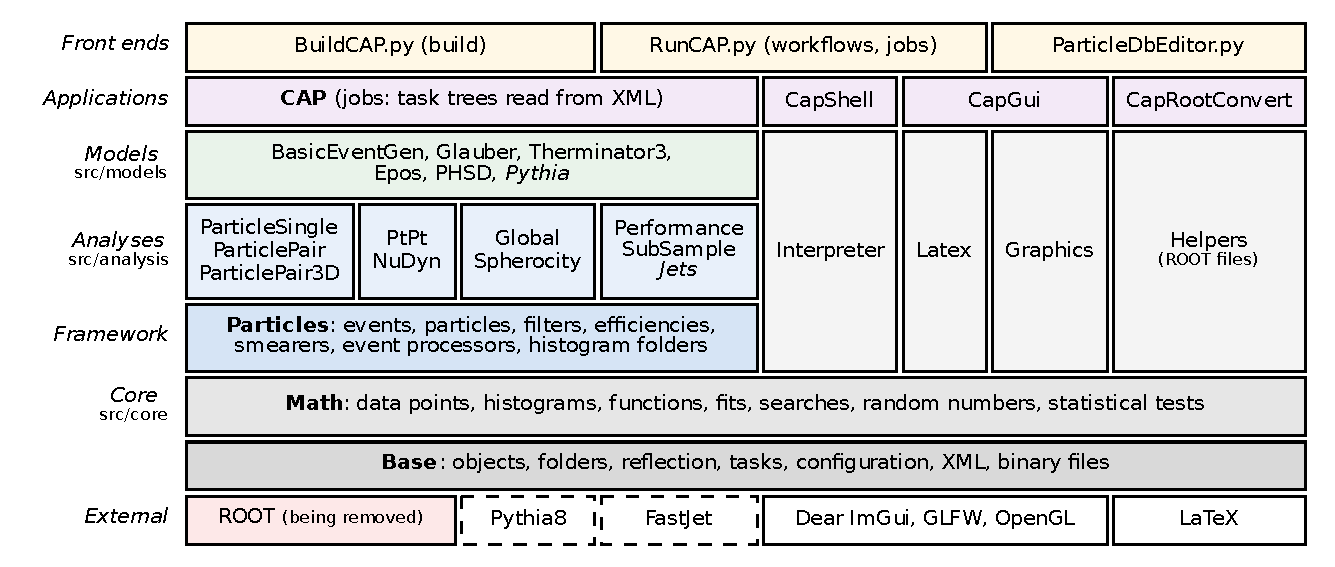
\includegraphics[width=\textwidth]{Layers}
  \caption{Layers of \CAP{}. Each layer uses only the layers below it; the libraries of the core on the right
  (Interpreter, Latex, Graphics, Helpers) use Math and Base, and not the analyses. Names in italics are optional
  modules; dashed boxes are optional external packages. The uses of ROOT that remain in the core and in the analyses are
  being removed (Section~\ref{sec:external}).}
  \label{fig:layers}
\end{figure}

% ---------------------------------------------------------------------------------------------------------------
\subsection{External software}
\label{sec:external}

\paragraph{Required.}
\CAP{} is built with CMake (3.5 or later) and a C++17 compiler; it is developed on macOS with Clang and built on Linux
with GCC. ROOT~\cite{Brun:1997pa} is still required to build it. Its remaining uses are listed here, as they are
the work left to make \CAP{} independent of ROOT: random numbers (\code{gRandom}) in a few tasks of the analyses and
models; system utilities and the \code{TString} class used by older code in Base; the reading of ROOT files by some
tasks; and the Glauber and Therminator3 models, written for earlier versions of \CAP{}. The conversion of
histograms from and to ROOT files (Helpers, \code{CapRootConvert}, and the reading of ROOT files by CapGui) will keep
using ROOT, but as an option (\code{CAP\_WITH\_ROOT\_FILES}). The front ends need Python~3.7 or later with tkinter.
\todo{\code{src/CMakeLists.txt} sets \code{CMAKE\_CXX\_STANDARD} to 14; the code is compiled as C++17 only because
the flags of ROOT ask for it. Set the standard to 17 before submission.}

\paragraph{Optional.}
The interfaces to Pythia~8~\cite{Bierlich:2022pfr} and Herwig~7~\cite{Bellm:2015jjp}, and the jet analyses, which
use FastJet~\cite{Cacciari:2011ma}, are built when asked for. CMake looks for each package in turn in a copy
distributed with \CAP{} (a folder \code{pythia8*}, \code{Herwig*} or \code{fastjet*} in the \CAP{} folder or in
\code{external}, or an installation \code{../Herwig/install} or \code{../Fastjet/install} next to the \CAP{} folder),
at the location given by an environment variable, and through the configuration tool of the package
(\code{pythia8-config}, \code{Herwig-config}, \code{fastjet-config}), or uses the location given explicitly. A LaTeX installation with \code{dvisvgm} is used, when
present, to typeset the texts of the figures (Section~\ref{sec:graphicscore}), and \code{pdflatex} to compile the
presentations; without them, texts are drawn with plain fonts. CapShell uses the \code{editline} library, when
present, for line editing and history.

\paragraph{Distributed with \CAP{}.}
CapGui is built on Dear ImGui~\cite{DearImGui} and GLFW, whose sources are in \code{external} and are compiled with
\CAP{}, and on OpenGL, which every desktop system provides; the texts typeset by LaTeX are rasterised for the screen with NanoSVG. Nothing else needs to be
installed to build the interface.

% ---------------------------------------------------------------------------------------------------------------
\subsection{Building: BuildCAP.py}
\label{sec:build}

\CAP{} is built with CMake, in a build folder of the \CAP{} folder, and installed in its folders \code{lib} and
\code{bin}. The script \code{BuildCAP.py} is a window from which the build is configured and run (Fig.~\todo{screenshot}).
It lists the core modules, always built, and the optional modules (Therminator3, Latex, Graphics, CapGui, the
conversion of ROOT files, Jets, Epos, PHSD, Pythia and Herwig), each with a check box, together with the locations of ROOT and of
the external packages; a button shows which installation of each package CMake will use. A toolbar chooses the build
folder, the build type, the number of parallel jobs, and whether to install, and the output of CMake and make is shown
in the lower half of the window and can be saved. Each command is printed before it runs, and the same build is made
from a terminal with
\begin{verbatim}
source SetupCAP.sh
cmake -S src -B build -DCAP_WITH_PYTHIA8=ON -DCAP_PYTHIA8_DIR=/opt/pythia8   # options as needed
make -C build -j8 install
\end{verbatim}
\code{BuildCAP.py -{}-print-commands} prints the commands of the saved settings without opening the window. Several build
folders can coexist, for instance one with Pythia and one without, or a release and a debug build. The environment
of \code{SetupCAP.sh} (the paths of \CAP{}, its libraries, its programs, its database and its projects) is set for the
commands, verbatim that the window works without a prepared shell. After a build, \code{ctest} runs the tests of the
modules: the test programs of Base, Math, Graphics, Latex, Interpreter, Helpers and Therminator3, and the tests of
the Python front ends.

% ---------------------------------------------------------------------------------------------------------------
\subsection{Running: RunCAP.py}
\label{sec:run}

\paragraph{Workflows.}
An analysis is described by a workflow file (Section~\ref{sec:xml}), which \code{RunCAP.py} composes, checks and
runs (Fig.~\todo{screenshot}). Its window has four parts. The workflow editor lists, on the left, the task classes of
the current build, read from their XML templates (which are regenerated when the program or the libraries are newer
than them), and on the right the tasks of the workflow; tasks are added, removed, ordered and nested, a nested task
being a subtask of the task above it, such as a generator and the analyzers inside an event iterator. A task can be
added several times, each copy with its own parameters. The filter editor defines the event and particle filters, the
efficiencies and the smearers of the workflow once, by their conditions or their parameters; they are created at the
start of the job by a filter-creator task, and each task chooses those it uses by name (Section~\ref{sec:filters}).
The task list shows, for each task in the order of execution, the filters it uses, its number of histogram folders,
and the first problem found in its configuration. A double click opens the window of a task, with its general
settings (name, report level, filters, efficiencies, particle databases, parameters) and its histograms: for each list
of folders, whether it is used, created, imported or exported, the prefix of the names of the folders, and either one
binning for all the folders or a binning per folder. The fields check the type of the values they accept. The values
read from a workflow file are checked against the templates, so that a misspelled or obsolete parameter is reported
when the file is loaded.

\paragraph{Stages and jobs.}
A workflow has up to three stages, which are the phases of Section~\ref{sec:phases}: event processing, derived
histograms and balance functions. Each stage is run as a job of its own,
\begin{verbatim}
bin/CAP <stage task> <directory of the workflow>/ <workflow file> <output directory>/
\end{verbatim}
the stages running one after the other, each reading the output file of the previous one. The derived-histogram stage is
made by \code{RunCAP.py} from the analyzers of the first stage, the first time it is shown: each analyzer gets its
calculator, with the same filters and histogram settings, so that the folders of the two jobs match. The output of
\CAP{} is shown as it runs, can be saved, and a job can be stopped. The same workflow file is run without the
window, on a cluster for instance, with the command above, which \code{RunCAP.py -{}-print-command} prints;
\code{RunCAP.py -{}-check} checks a file against the templates.
\todo{the scripts of \code{Grid} that submit many jobs and combine their outputs (Section~\ref{sec:subsample}).}

% Section: The core: Base
\section{The core: Base}
\label{sec:base}

The Base library (\code{src/core/Base}) provides what every other part of \CAP{} builds on: the base class of named
objects and its reporting of messages, exceptions, a tree of named objects of any type, a registry of classes for
reflection, the configuration of tasks, the binary file format, and the reading and writing of XML formatted data. Its classes
depend only on the C++ standard library, with the exception of few helper optional  functions used  to load and export data from ROOT files.

% ---------------------------------------------------------------------------------------------------------------
\subsection{Object model}
\label{sec:objects}

\paragraph{Objects and messages.}
Most classes of \CAP{} derive from \code{Object}, which gives them a name, a title, a class name and a version
index. Each object has a minimum report level, one of the severities \code{TRACE}, \code{DEBUG}, \code{INFO},
\code{WARNING}, \code{ERROR} and \code{FATAL}; a message is printed only if its severity is at least that level, with
a header naming the class, the object and the function that issued it. The report level of each task is set in its
configuration, so that the messages of one part of a workflow can be followed without those of the others. All
exceptions of \CAP{} derive from \code{Exception}, itself a \code{std::exception}, and record a message, the function
that threw them and their class (file, configuration, histogram, mathematical domain, and so on).

\paragraph{Folders.}
A \code{Folder} is a container of named objects of any type and of sub-folders, forming a tree. The folder owns its
objects: copying a folder copies them, and removing or replacing an object deletes it. Objects are reached by name or
by path through the sub-folders, \code{get<Histogram>("PtPt/pairs/n2")}, and a folder can be navigated like a file
system, with \code{cd()} and relative or absolute paths. Typed access works through the base classes of the objects,
so that a histogram is found as a \code{Histogram}, a \code{DataPoints} or an \code{Object}. Two folders of the same
structure can be added or subtracted entry by entry, for every type that has a sum, to combine the results of
several jobs; sub-samples are combined by a dedicated task, which averages them and takes their spread as the
uncertainty (Section~\ref{sec:subsample}). Folders are the unit of input and output of the analyses: each job writes the
histograms of its tasks to a folder, with one sub-folder per task and one per combination of filters
(Section~\ref{sec:folders-analysis}), and saves it to a file (Section~\ref{sec:binary}).

\paragraph{Reflection.}
Earlier versions of \CAP{} relied on the dictionaries of ROOT to create objects from their class names, which is
how the tasks of a workflow are instantiated from an XML file. \CAP{}~8 has its own run-time registry of classes
(\code{Reflection.hpp}), written in standard C++17. A class is described once in C++: its bases, its constructors,
its data members and properties, and its member functions, overloads and inherited functions included. The registry
then finds classes by name and lists them by base class, creates objects with any of their constructors, reads and
writes their properties, and calls their member functions by name:
\begin{verbatim}[language=C++]
const ClassInfo * h = Registry::instance().find("Histogram");
Value g    = Registry::instance().find("MersenneTwister")->create({ 12345 });
Value hist = h->create({ "h", "Gaussian numbers", 40, -4.0, 4.0 });
for (int k=0; k<10000; k++) hist.call("fill", { g.call("gauss", { 0.5, 1.0 }) });
hist.call("nBins", { 0 });   // a member function of Partition, a base of Histogram
\end{verbatim}
All the task classes are registered, one line each, so that workflows create their tasks by class name. The same
registry serves the command-line interpreter, CapShell (Section~\ref{sec:capshell}). Its descriptions are written by
hand today; they are meant to be generated by the static reflection of C++26 once the compilers used by \CAP{}
support it.

\paragraph{Tasks.}
The work of a job is done by a tree of tasks (\code{Task}). A task goes through a fixed life cycle: its default
configuration is defined (\code{setDefaultConfiguration()}), the configuration is read (\code{configure()}), the task
is initialised once, executed repeatedly, typically once per event, and finalised. A task owns its subtasks and
passes each step of the cycle on to them, after doing its own part; an event iterator, for instance, executes a
generator and then the analyses for each event. Tasks are created from their class names through the registry,
and their parameters, subtasks included, are read from XML (Section~\ref{sec:xml}).

% ---------------------------------------------------------------------------------------------------------------
\subsection{Binary data model}
\label{sec:binary}

\CAP{}~8 stores its objects in its own binary format, independent of ROOT. The format was designed to be compact,
portable between platforms and compilers, robust against corrupted or truncated files, and readable by later
versions of the code.

\paragraph{Records.}
A file is a sequence of records, one per object. Each record is
\begin{center}
  \small
  \begin{tabular}{@{}lll@{}}
    \toprule
    Field & Size & Content \\
    \midrule
    tag & 4 bytes & \code{CAP} followed by one letter identifying the class \\
    version & 1 byte & format version of the payload \\
    length & varint & number of bytes of the payload \\
    payload & length & the name of the object, then the data of its class \\
    checksum & 4 bytes & CRC-32 of the payload \\
    \bottomrule
  \end{tabular}
\end{center}
Integers are written as variable-length integers (LEB128: seven bits per byte, one byte below 128), signed integers
after a zigzag mapping that keeps small negative numbers short, floating-point numbers as their IEEE~754 bit patterns,
and every multi-byte value in little-endian order, byte by byte, so that files are the same on every platform.
Strings are written as their length followed by their bytes. Arrays of doubles are written densely or sparsely
(only the non-zero values, each with the gap in index since the previous one), whichever is smaller, and are restored
exactly. The CRC-32 checksum (the polynomial of zip and png) detects corrupted data, and every read is checked against
the bounds of the record, so that a damaged file is refused with an exception rather than read wrongly.
Table~\ref{tab:tags} lists the classes that are stored this way.

\begin{table}[t]
  \centering
  \caption{Classes stored in the CAP binary format, with their record tags.}
  \label{tab:tags}
  \small
  \begin{tabular}{@{}llll@{}}
    \toprule
    Tag & Class & Tag & Class \\
    \midrule
    \code{CAPO} & \code{Folder} (holds the records of its entries) & \code{CAPF} & \code{ScalarField} \\
    \code{CAPH} & \code{Histogram} & \code{CAPM} & \code{Matrix} \\
    \code{CAPQ} & \code{Profile} & \code{CAPV} & \code{VectorND} \\
    \code{CAPD} & \code{DataPointsVector} & \code{CAP2}, \code{CAP3} & \code{Vector2D}, \code{Vector3D} \\
    \code{CAPK} & \code{DataPointColumns} & \code{CAPL} & \code{VectorLorentz} \\
    \code{CAPP}, \code{CAPT}, \code{CAPN} & \code{DataPoint2D}, \code{3D}, \code{ND} & \code{CAPR}, \code{CAPI} & \code{Parameter}, \code{LongParameter} \\
    \code{CAPB} & \code{Table2D} & & \\
    \bottomrule
  \end{tabular}
\end{table}

\paragraph{Histograms.}
The payload of a histogram holds its name and title, then its rank and, for each axis, the number of bins, the range
and the title; then the number of non-empty bins and, for each of them, the gap in global index since the previous
non-empty bin, the number of entries, the average value and its uncertainty; then the labels of the bins and the fits
attached to the histogram. Empty bins are not written at all, and a filled bin takes about ten bytes, so that the
large and sparse histograms of the pair analyses stay small on disk. The content of the histogram is restored
exactly.

\paragraph{Functions and fits.}
A function is stored as part of the fits attached to data points, a histogram or another function. A fit record holds
the name under which the class of the fitted function is registered (Section~\ref{sec:functions}), its number of
parameters and its rank, the name, value, type and bounds of each parameter, the label and result of the fit, its
range, and its regions. When the file is read, the function is recreated by name through the registry and given its
parameters, so that any registered class, a composite registered under a name included, is read back. A fit whose
class is not registered by the program reading the file is skipped, and the number of fits skipped is returned to
the caller.
\todo{decide whether functions should also be stored as objects of their own in folders, not only as fits.}

\paragraph{Folders and files.}
A folder is stored as one \code{CAPO} record whose payload holds the records of its entries, sub-folders included,
so that a whole tree of results is one record. When a file is read, each record is rebuilt as an object of its
class through a registry of types, in which the Math library registers its classes when it is loaded; programs add
their own with \code{Folder::registerType<T>()}. A \code{CapFile} holds one or several folders. It can be read eagerly,
or lazily: the tree of folders is then built at once, with the names and types of all the objects, and each object is
decoded only when it is first used, which makes it quick to open a large file and look at a few of its histograms.
The checksums of a lazily read file are verified when it is opened, so a corrupted file is still refused at once.

\paragraph{Versions.}
Each class writes its records with its current format version and reads every version up to that one: histograms,
for instance, are at version~4 and still read the earlier versions. Records of classes a program does not know are
skipped, so that one file can hold objects of many classes. Additions that older code can ignore are placed at the end
of a block: the regions of a fit (Section~\ref{sec:fitting}) are written after its range, and only when the fit has
some, so that files written with regions are still read, without them, by earlier versions of \CAP{}~8.

% ---------------------------------------------------------------------------------------------------------------
\subsection{Configuration in XML}
\label{sec:xml}

\paragraph{Properties and configurations.}
The parameters of the tasks are properties: named values whose names are paths of components separated by colons,
such as \code{PtPt:HISTOGRAM:pt\_nbins}. Values are stored as text and read as booleans, integers, floating-point
numbers or strings; a property keeps the type of its default value, so that a value of the wrong type is detected when
a configuration is read. A key matches a property of the same name or one whose name ends with it, so that a task reads
its parameters with keys relative to its own name. A \code{Configuration} adds numbered keys, lists of values such as
the particle filters of a task (\code{PARTICLE\_FILTER\_0}, \code{PARTICLE\_FILTER\_1}, \dots).

\paragraph{XML.}
The configuration of a task maps to an XML element: the task is a \code{TASK} element whose name, class and severity
are attributes, each component of a key but the last becomes a \code{GROUP} element, the last one a \code{PARAMETER}
element holding the value and its type, and the subtasks are nested \code{TASK} elements. The XML classes of Base
(\code{XmlDocument}, \code{XmlElement}, \code{XmlReader}, \code{XmlWriter}) need nothing but the standard library. The
reader is a non-validating parser that loads no external content and does not recurse, so that malformed or deeply
nested input is reported with its line and column instead of being read wrongly; the writer streams large documents
without building them in memory first.

\paragraph{Templates.}
There is no fixed dictionary of parameters. Each class defines its own in its function
\code{setDefaultConfiguration()}, which lists its parameters with their default values and types. Run with the option \code{-{}-xml-templates}, the \code{CAP} program writes this
template for every registered task class, one XML file per class in \code{DB/Templates}. The workflow editor \code{RunCAP.py}
(Section~\ref{sec:run}) builds its task dialogs from these templates, and the values read from a workflow file are
checked against them; a parameter that is not in the template of its class is reported.

\paragraph{Workflow files.}
A workflow file has a \code{CAP} root element with one top-level \code{TASK} element per stage of the analysis (event
processing, derived histograms, balance functions), marked by a \code{stage} attribute, each with the job settings
(output and input files) and its tree of tasks. A \code{RUNCAP} element at the end holds what the editor needs to rebuild
its own view: the definitions of the event and particle filters, the generators and particle databases used, and the
histogram settings shared between tasks. An excerpt:
\begin{widetext}
\begin{verbatim}[language=XML]
<CAP version="1">
  <TASK name="Workflow" class="CAP::Task" severity="INFO" stage="EventProcessing">
    <GROUP name="JOB">
      <PARAMETER name="OUTPUT_FILE" type="string">RunAna.cap</PARAMETER>
    </GROUP>
    <TASK name="RunAnalysis" class="CAP::EventIterator" severity="INFO">
      <TASK name="PythiaEventGenerator" class="CAP::PythiaEventGenerator"> ... </TASK>
      <TASK name="ParticlePairAnalyzer" class="CAP::ParticlePairAnalyzer"> ... </TASK>
    </TASK>
  </TASK>
  <TASK name="DerivedHistos" class="CAP::Task" stage="DerivedHistos"> ... </TASK>
  <RUNCAP version="1">
    <OBJECT kind="PARTICLE_FILTER" name="PiP" title="#pi^{+}">
      <CONDITION subtype="PDG" form="value" minimum="211" maximum="211" />
    </OBJECT>
    ...
  </RUNCAP>
</CAP>
\end{verbatim}
\end{widetext}
% Section: The core: Math
\section{The core: Math}
\label{sec:math}

The Math library (\code{src/core/Math}) holds the numerical objects of \CAP{}: data points and histograms, functions,
fits, extremum searches, random numbers, statistical tests and linear algebra. It replaces the parts of ROOT that
earlier versions of \CAP{} relied on (histograms, \code{TF1}, \code{TGraph}, \code{TProfile}, the fitters and
\code{gRandom}); its sources use only the Base library and the C++ standard library, and include no ROOT header. Its classes are arranged in
eight folders: \code{Basic} (constants, special functions, integration, interpolation, statistics), \code{Data},
\code{Functions}, \code{Fitting}, \code{Search}, \code{Random}, \code{StatisticalTests} and \code{LinearAlgebra}.
Figure~\ref{fig:hierarchy} shows the class hierarchy of the functions and of the data.

\begin{figure}[t]
  \centering
  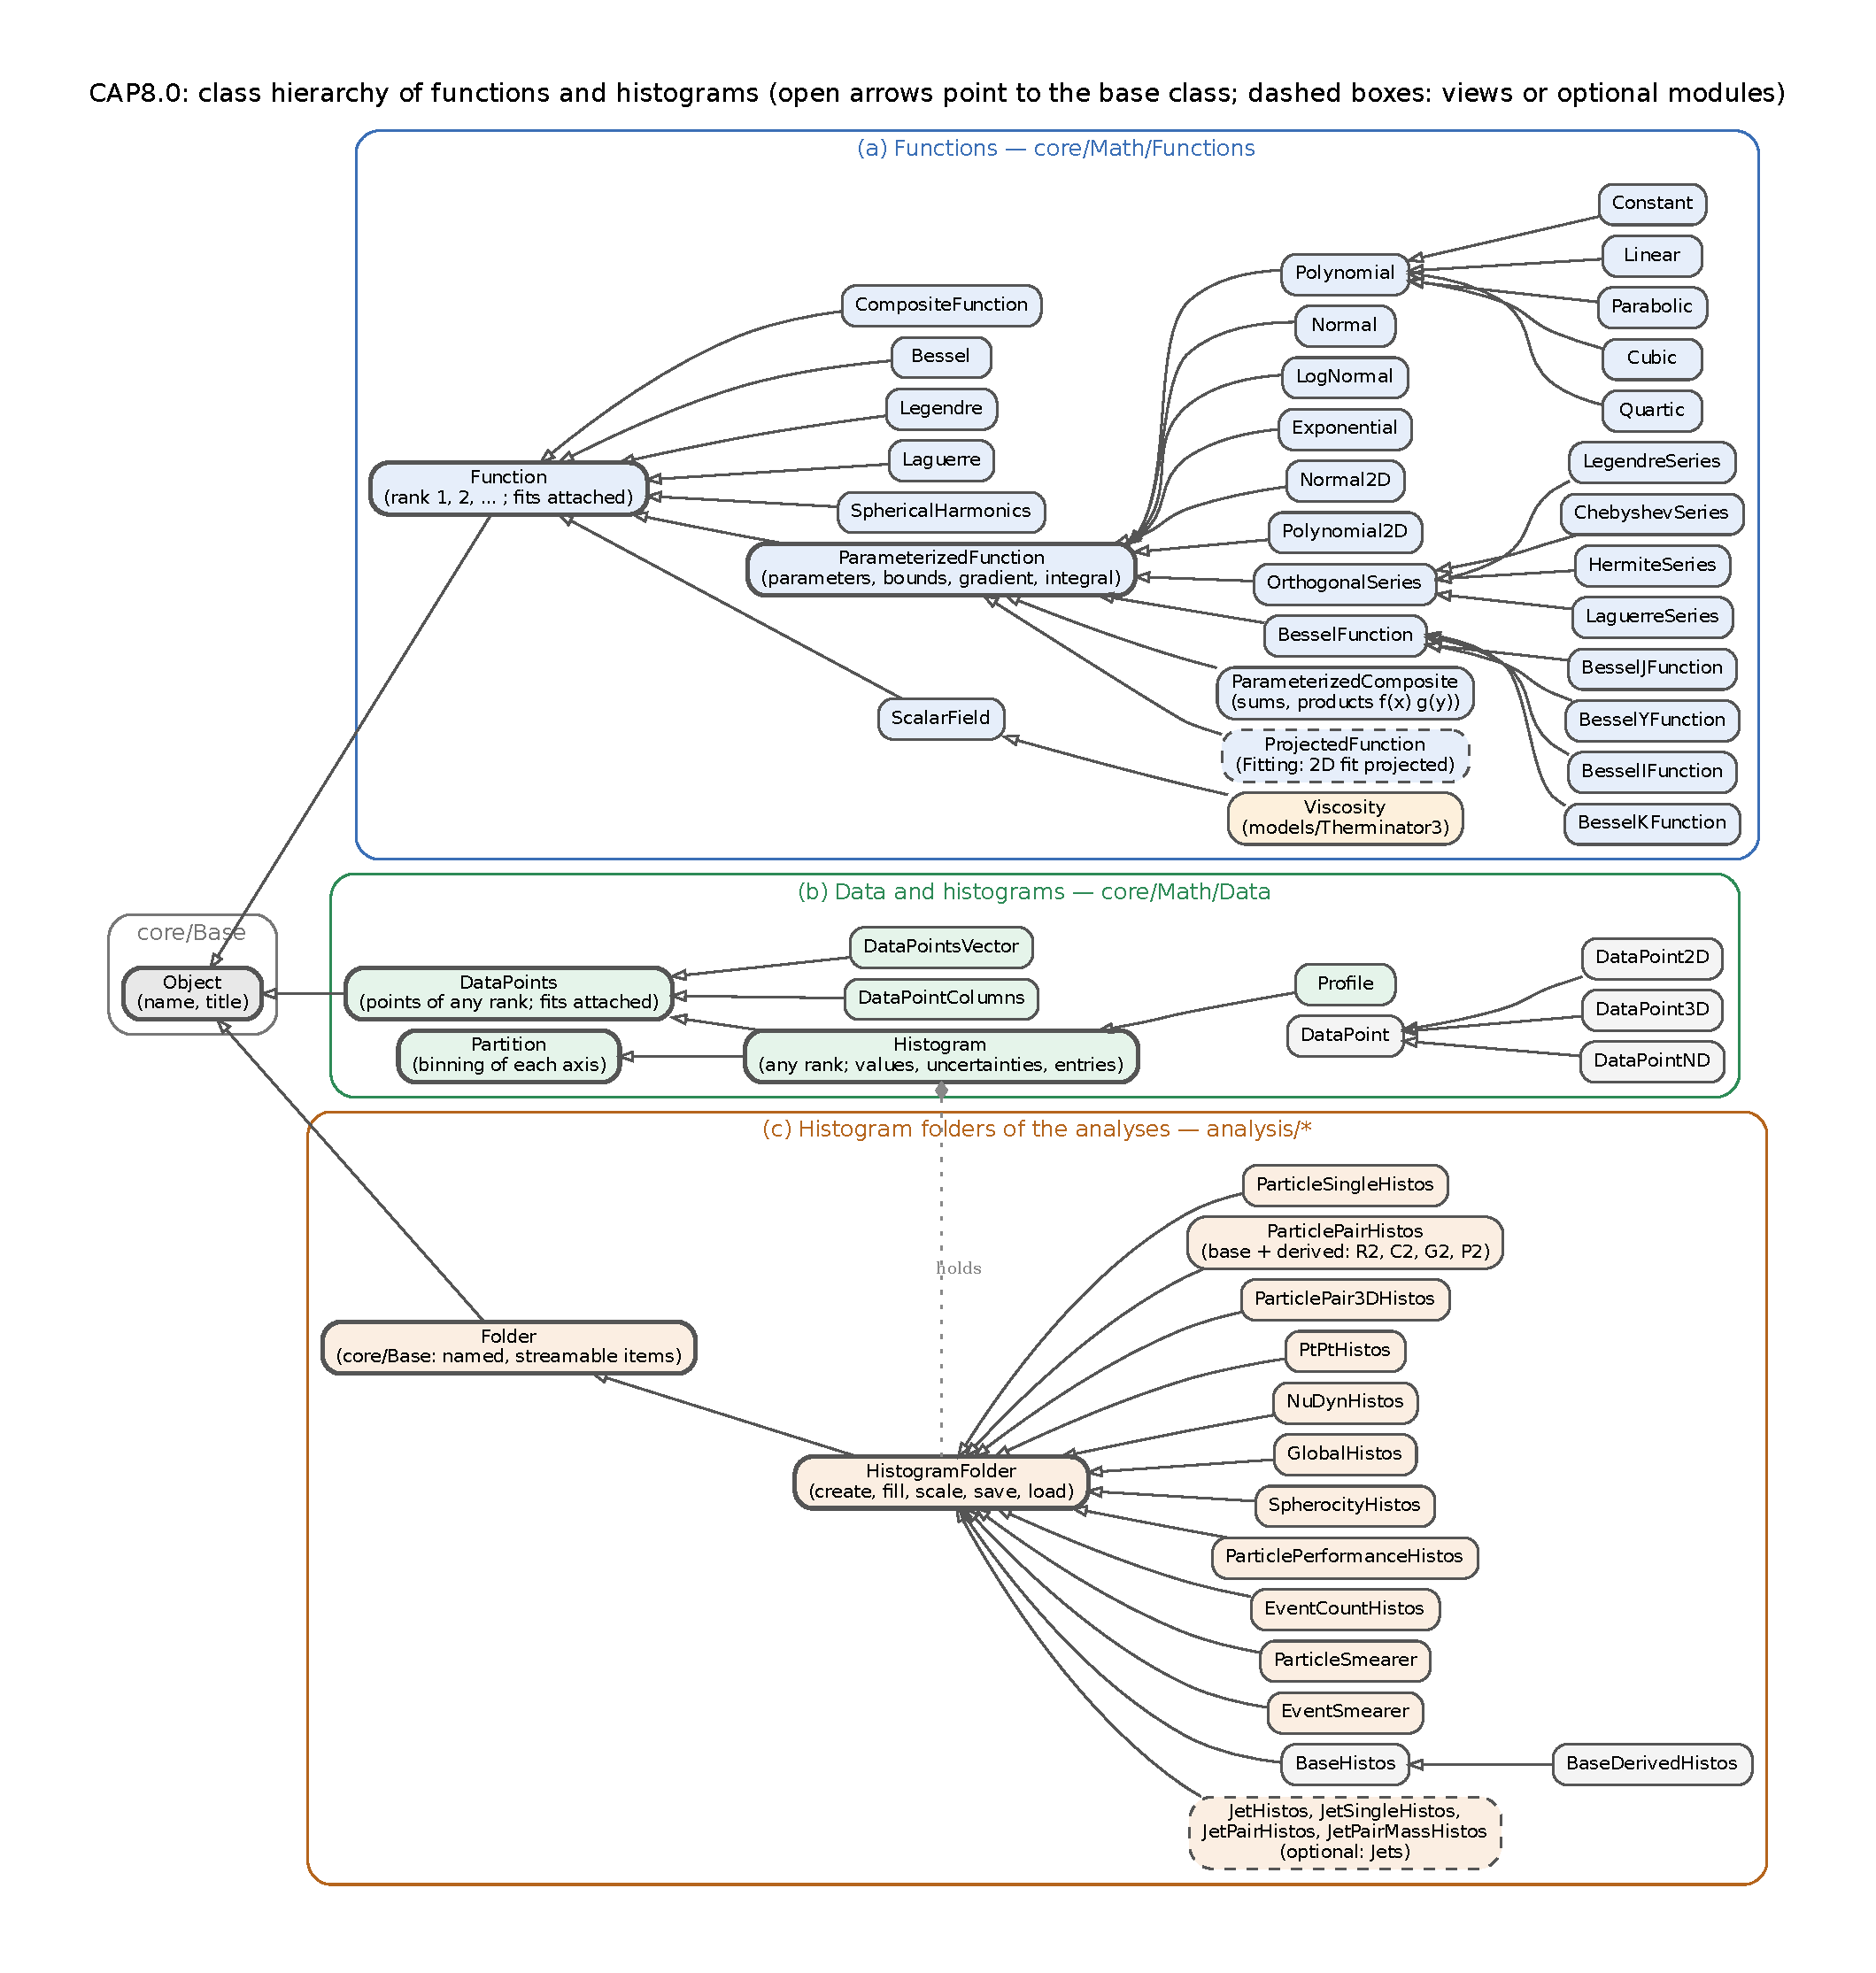
\includegraphics[width=\textwidth]{ClassHierarchy}
  \caption{Class hierarchy of the functions and histograms of \CAP{}~8. Open arrows point to the base class.
  (a)~Functions (\code{core/Math/Functions}); (b)~data points and histograms (\code{core/Math/Data});
  (c)~histogram folders of the analyses (\code{src/analysis}). Dashed boxes are views (\code{ProjectedFunction})
  or optional modules (Jets).}
  \label{fig:hierarchy}
\end{figure}

% ---------------------------------------------------------------------------------------------------------------
\subsection{Data points and histograms}
\label{sec:data}

\paragraph{Data points.}
\code{DataPoints} is the abstract base of every set of measured or computed values. A set has a rank $r$, the number
of its coordinates, and each of its points has coordinates $\mathbf{x}_i = (x_{i,1},\dots,x_{i,r})$ with their
uncertainties, a value $y_i$, a statistical uncertainty $\sigma_i$ and a systematic uncertainty $s_i$. The interface
(\code{coordinatesAt()}, \code{valueAt()}, \code{statErrorAt()}, \code{sysErrorAt()}) is the same for every rank, so
that the fitter, the extremum searches and the graphics work on any set of points without knowing how it is stored.
Two classes store points: \code{DataPointsVector}, a vector of point objects (\code{DataPoint2D},
\code{DataPoint3D}, \code{DataPointND}), and \code{DataPointColumns}, one vector per quantity, which is more compact
for large sets. A set of points also holds the fits made to it (Section~\ref{sec:fitting}).

\paragraph{Partitions.}
The binning of a histogram is a \code{Partition}: a regular partition of a space of any rank, built one axis at a
time. Axis $k$ is divided into $n_k$ bins of equal width over $[a_k, b_k)$. A bin is addressed by its indices
$(i_0, i_1, \dots)$ along the axes, by the coordinates of a point inside it, or by a single global index
\begin{equation}
  g = i_0 + n_0\,\bigl(i_1 + n_1\,(i_2 + \dots)\bigr), \qquad 0 \le g < \prod_k n_k ,
\end{equation}
which is how the bins are stored. Nothing in the classes is specific to one, two or three dimensions: the pair
analyses of Section~\ref{sec:observables} use histograms of rank 2, the three-dimensional pair analysis
histograms of rank 3, and nothing prevents higher ranks.

\paragraph{Histograms.}
\code{Histogram} derives from both \code{DataPoints} and \code{Partition}: a histogram is a set of points, one per bin,
whose coordinates are the centres of the bins, and its binning is a partition. Each bin $g$ stores three numbers:
the number of entries $n_g$ (the number of fills), the average value per entry $a_g$, and the uncertainty $u_g$ of
that average. The bin value and its uncertainty are
\begin{equation}
  y_g = n_g\, a_g, \qquad \sigma_g = n_g\, u_g .
\end{equation}
Filling with a weight $w$ adds $w$ to the value and $w^2$ to its squared uncertainty. Arithmetic (sums,
differences, products, ratios, scaling) acts on the bin values and propagates the statistical uncertainties of
uncorrelated operands; bins where a result is undefined, for instance a ratio with an empty denominator, are left
empty. Values are stored in single or double precision, chosen per histogram, so that the large pair histograms of
an analysis take half the memory when single precision suffices.

The histogram library includes the operations the analyses need on their histograms: integrals over ranges,
projections and reductions (for example from $(\eta_1,\varphi_1,\eta_2,\varphi_2)$ to $(\Delta\eta,\Delta\varphi)$),
symmetrisation, shifts of the $\Delta\varphi$ range, and the computation of the correlation functions of
Section~\ref{sec:observables}: products of single-particle densities, cumulants $C_2$, normalised cumulants $R_2$,
the correlators $\avg{\Delta\pT\Delta\pT}$ and $G_2$, balance functions, and the factorial moments and $\nudyn$ of
multiplicity distributions.

\paragraph{Profiles.}
\code{Profile} derives from \code{Histogram} and holds, in each bin, the weighted mean of a quantity and its
uncertainty. Each bin keeps the sums of the weights $w$, of their squares, of $w v$ and of $w v^2$; the bin value is
the mean and the bin uncertainty the standard error of the mean. Adding two profiles combines these sums, so
merging the profiles of several jobs or sub-samples gives the exact weighted mean.

% ---------------------------------------------------------------------------------------------------------------
\subsection{Functions}
\label{sec:functions}

\paragraph{Functions and parameterised functions.}
\code{Function} is the abstract base of real functions of $r$ real variables, $f(x_1,\dots,x_r)$; $r$ is its rank.
A function is evaluated with one, two or three arguments, or with a vector of arguments, and a call with the wrong
number of arguments throws an exception. \code{ParameterizedFunction} adds a list of parameters,
$f(\mathbf{x};\mathbf{p})$. Each \code{Parameter} has a name, a value, a range and a type that says how it may vary in
a fit: free, fixed, or bounded from below, above or both. A parameterised function provides its gradient
$\nabla_{\mathbf{x}} f$ and its integral over a box; the defaults are numerical (finite differences for the gradient, adaptive Simpson rules for the integrals) and the
functions of the library override them with analytical expressions where these exist. For rank one, the derivative
$f'(x)$ and the mean of $x$ weighted by $f$ over a range are also available.

\paragraph{The library.}
Table~\ref{tab:functions} lists the parameterised functions of \CAP{}. Polynomials of high degree are badly
conditioned in fits; the series of orthogonal polynomials map the range of a fit onto the natural domain of the
polynomials (for example $[-1,1]$ for Legendre and Chebyshev polynomials), where they are nearly orthogonal, and
being linear in their coefficients, their least-squares coefficients are obtained exactly. The library also includes
special functions without parameters (Bessel, Legendre and Laguerre functions, spherical harmonics) and scalar
fields, functions of any rank defined by their values on a regular mesh and interpolated multilinearly, which
Therminator3 uses for its chemical potentials and viscosity (Section~\ref{sec:therminator}).

\begin{widetext}
\begin{table}[t]
  \centering
  \caption{Parameterised functions of \CAP{}~8 (\code{core/Math/Functions}).}
  \label{tab:functions}
  \small
  \begin{tabular}{@{}lll@{}}
    \toprule
    Class & Rank & Form \\
    \midrule
    \code{Polynomial} (\code{Constant} to \code{Quartic}) & 1 & $\sum_{k=0}^{n} c_k x^k$ \\
    \code{Normal} & 1 & $A\, e^{-(x-\mu)^2/2\sigma^2}$ \\
    \code{LogNormal} & 1 & $\dfrac{A}{x\sigma\sqrt{2\pi}}\, e^{-(\ln x-\mu)^2/2\sigma^2}$ \\
    \code{Exponential} & 1 & $a\, e^{b x}$ \\
    \code{LegendreSeries}, \code{ChebyshevSeries} & 1 & $\sum_{k=0}^{N} c_k P_k(t)$, $t\in[-1,1]$ \\
    \code{HermiteSeries} & 1 & $\sum_{k=0}^{N} c_k H_k(t)$ \\
    \code{LaguerreSeries} & 1 & $\sum_{k=0}^{N} c_k L^{\alpha}_k(t)$ \\
    \code{BesselJFunction} (and \code{Y}, \code{I}, \code{K}) & 1 & $A\, Z_n\bigl(k(x-x_0)\bigr)$ \\
    \code{Normal2D} & 2 & $A\exp\!\left[-\dfrac{u^2 - 2\rho u v + v^2}{2(1-\rho^2)}\right]$ \\
    \code{Polynomial2D} & 2 & $\sum_{i+j\le N} c_{ij}\, t^i s^j$ \\
    \code{ParameterizedComposite} & any & $\sum_k f_k(\mathbf{x};\mathbf{p}_k)$, or $f(x)\,g(y)$ \\
    \bottomrule
  \end{tabular}
  \smallskip
  \raggedright\footnotesize In \code{Normal2D}, $u=(x-\mu_x)/\sigma_x$ and $v=(y-\mu_y)/\sigma_y$. In \code{Polynomial2D} and the
  series, $t$ and $s$ are $x$ and $y$ mapped onto the domain of the polynomials.
\end{table}
\end{widetext}

\paragraph{Composite functions.}
A \code{ParameterizedComposite} is a sum of parameterised functions, $f = \sum_k f_k(\mathbf{x};\mathbf{p}_k)$, whose
parameters are those of all its components, named after the label of each component (for example
\code{signal.mean}), or a product of functions of separate variables, such as $f(x)\,g(y)$, a function of two
variables made of two of one. Its derivatives and integrals are those of its components, analytical when theirs
are. A composite can be fitted, copied and stored with its fits like any other function:
\begin{widetext}
\begin{verbatim}[language=C++]
CAP::MATH::ParameterizedComposite model;
model.add("signal",     CAP::MATH::Normal(100.0, 0.0, 1.0));
model.add("background", CAP::MATH::Linear(10.0, 0.0));
CAP::MATH::FunctionRegistry::registerComposite("Gauss+Linear", model);
\end{verbatim}
\end{widetext}
\paragraph{The function registry.}
\code{FunctionRegistry} maps names to classes of parameterised functions and makes new functions by name. It is how
fits are read back from files, which store the name of the class of the fitted function and its parameters, and
how the Fit window of CapGui offers its functions. Programs register their own classes, and composites registered
under a name are kept in a file shared by the programs and CapGui.

% ---------------------------------------------------------------------------------------------------------------
\subsection{Fitting}
\label{sec:fitting}

\paragraph{Statistics.}
A fit finds the parameters $\mathbf{p}$ of a function that minimise a statistic $S(\mathbf{p}) = -2\ln L$, up to a
constant (\code{Likelihood}). Three statistics are provided. For data with Gaussian uncertainties, $S$ is the
$\chi^2$,
\begin{equation}
  \chi^2(\mathbf{p}) = \sum_{i} \frac{\bigl(y_i - f(\mathbf{x}_i;\mathbf{p})\bigr)^2}{V_i},
  \qquad V_i = \sigma_i^2 + s_i^2 + \sum_{k} \left(\frac{\partial f}{\partial x_k}\right)^{\!2} \sigma_{x_k,i}^2 ,
\end{equation}
where the systematic uncertainties $s_i$ and the effective variance from the coordinate uncertainties are included
on request (for rank one, the covariance of $x$ and $y$ is included as well). Points without an uncertainty, such as
the empty bins of a histogram, are left out. For histograms with few entries per bin, the binned Poisson likelihood
ratio of Baker and Cousins~\cite{Baker:1983tu},
\begin{equation}
  S_{\mathrm{P}}(\mathbf{p}) = 2 \sum_{g} \left[ f_g - n_g + n_g \ln\frac{n_g}{f_g} \right],
\end{equation}
is unbiased where the $\chi^2$ is not, includes the empty bins, and is asymptotically $\chi^2$-distributed. For
individual events, the unbinned likelihood takes the function as the density of the events over a range $\Omega$,
\begin{equation}
  S_{\mathrm{U}} = -2\sum_{i} \ln\frac{f(\mathbf{x}_i;\mathbf{p})}{N(\mathbf{p})}, \qquad
  S_{\mathrm{E}} = 2N(\mathbf{p}) - 2\sum_{i} \ln f(\mathbf{x}_i;\mathbf{p}), \qquad
  N(\mathbf{p}) = \int_{\Omega} f(\mathbf{x};\mathbf{p})\, d\mathbf{x},
\end{equation}
without and with extension ($S_{\mathrm{E}}$, where $N$ is the expected number of events and the amplitude is
fitted). For histograms whose bins are wide compared to the structures fitted, the function can be compared to its
average over each bin, computed with a three-point Gauss--Legendre rule along each axis, rather than to its value at
the centre of the bin.

\paragraph{Ranges and regions.}
A fit uses the points in a selection (\code{FitSelection}): a box, $a_k \le x_k \le b_k$ for each variable, regions
included, and regions excluded. A region is a set of intervals along some of the variables, the others not being
restricted, so that it is a band, a slab or a box. A point, or the centre of a bin, is used if it is in the box, in at
least one included region (if there is any), and in no excluded region. Excluding a region leaves out a peak or a
dead area; including two regions fits two sidebands. For an unbinned fit, the normalisation $N(\mathbf{p})$ is the
integral over the selection: the box is split into cells at the ends of the intervals of the regions, each cell is
either wholly in or wholly out of the selection, and $N$ is the sum of the integrals over the cells that are in.

\paragraph{Minimisation.}
The default method is Levenberg--Marquardt. For a statistic made of residuals $r_i$ ($\chi^2$ and Poisson
likelihood, whose residuals are the pulls and the signed deviance residuals), each step solves
\begin{equation}
  \bigl(J^{\mathsf{T}}J + \lambda\,\mathrm{diag}(J^{\mathsf{T}}J)\bigr)\,\delta\mathbf{p} = -J^{\mathsf{T}}\mathbf{r},
\end{equation}
where $J_{ia} = \partial r_i/\partial p_a$ is computed by central differences (one-sided at a bound), and the damping
$\lambda$ grows tenfold until $S$ decreases and shrinks tenfold after each successful step. For the unbinned
likelihood, which is not a sum of squares, the same scheme is applied to the numerical gradient and curvature of
$S$. Fixed parameters keep their values, and bounded parameters stay within their bounds. When the starting values
are poor or $S$ has several minima, a global search (Section~\ref{sec:mathother}), such as differential evolution
over the bounds of the free parameters, runs first and Levenberg--Marquardt refines its result. Starting values can
also be estimated from the data in the selection for the common functions: moments for Gaussian peaks, a straight
line in $\ln y$ for an exponential, exact least squares for polynomials and series.

\paragraph{Uncertainties.}
The covariance of the free parameters at the minimum is $C = (J^{\mathsf{T}}J)^{-1}$ for a statistic made of residuals,
and $C = 2H^{-1}$ otherwise, $H$ being the curvature of $S$. It can be scaled by $\chi^2/\nu$ when the uncertainties
of the data are known only up to a factor. The result of a fit (\code{FitResult}) holds the values, uncertainties,
covariance and correlation matrices of the parameters, the statistic, the number of degrees of freedom $\nu$ and,
for the binned statistics, the $p$-value of the $\chi^2$ distribution, together with flags for convergence and for
parameters at a bound.

\paragraph{Bayesian fits.}
\code{BayesianFitter} samples the posterior distribution of the parameters,
\begin{equation}
  p(\mathbf{p}\,|\,\text{data}) \propto L(\mathbf{p})\,\prod_a \pi_a(p_a),
\end{equation}
with priors $\pi_a$ that are flat, uniform, Gaussian (for instance an earlier
measurement), log-uniform for a scale of unknown magnitude, or any log density. The sampler is an adaptive
Metropolis--Hastings algorithm: several chains (four by default) start near the starting values; during the burn-in
the size of the proposals adapts to a target acceptance of 0.25, and halfway through it their covariance becomes that
of the samples drawn so far, so that correlated parameters are sampled efficiently. The result gives, for each
parameter, its mean, spread, quantiles, credible intervals and mode, the covariance of the samples, and the
diagnostics of the chains: acceptance, effective sample size and $\hat{R}$.

\paragraph{Fits attached to the objects fitted.}
A fit is kept with the object it was made to, data points, a histogram or a function, as a \code{FitRecord}: a copy of
the fitted function at the best parameters, the result, a label, the box covered by the points used and the regions
of the selection. The records are written to and read from CAP files with the object (Section~\ref{sec:binary}),
the function being recreated through the registry, so that a fit made in a program is drawn and inspected in
CapGui, and the reverse. The residuals of a fit, $y_i - f(\mathbf{x}_i)$ or the pulls, are computed for the points
used, and the fits of rank two of a histogram can be projected onto either axis with the histogram:
\begin{verbatim}[language=C++]
CAP::MATH::Normal model(100.0, 0.0, 1.0);            // starting values
CAP::MATH::Fitter fitter(model, histogram);          // chi square by default
fitter.exclude(0, 4.5, 5.5);                         // leave a region out
CAP::MATH::FitResult r = fitter.fit();
histogram.addFit(fitter.record("gaussian"));         // saved with the histogram
\end{verbatim}

% ---------------------------------------------------------------------------------------------------------------
\subsection{Searches, random numbers, statistical tests and linear algebra}
\label{sec:mathother}

\paragraph{Extremum searches.}
\code{ExtremumSearch} finds the minimum or maximum of a function or of a set of data points over a domain with
bounds and excluded regions. Local methods (gradient, hill climbing, greedy) start from a point; global methods (scan,
simulated annealing, genetic algorithm, differential evolution, divide and conquer, explore--exploit) need a bounded
domain. A second method can refine the result of the first, a method can be run from several starting points, and
for histograms the extremum is placed between bins by a parabolic fit. The fitter uses these engines for its global
searches.

\paragraph{Random numbers.}
\code{RandomGenerator} draws the common distributions (Gaussian, exponential, Poisson, binomial, gamma, beta,
$\chi^2$, polynomial densities) from the uniform numbers of any engine; the engine provided is the Mersenne Twister
MT19937, whose state can be saved and restored to continue a sequence. New distributions derive from
\code{RandomDistribution} and work with every engine.

\paragraph{Statistical tests.}
Binomial, Poisson, Gaussian, Student $t$ and $\chi^2$ tests, the compatibility of two histograms, and the
Kolmogorov--Smirnov test are provided, with one- or two-sided alternatives, together with the cumulative
distributions they need. Upper tails are computed directly, so that small $p$-values keep their precision.

\paragraph{Linear algebra and kinematics.}
\code{Matrix} provides the dense matrices of the fits (products, inverses, determinants), and \code{Vector2D},
\code{Vector3D}, \code{VectorND} and \code{VectorLorentz} the vectors and four-vectors of particle kinematics, with
the $(+,-,-,-)$ metric and $c=1$.

\todo{decide whether to add a short paragraph on Basic (integration, interpolation, robust moments) and a figure
of a fit with an excluded region drawn by CapGui.}

% Section: The core: Graphics, Latex and Interpreter
\section{The core: Graphics, Latex and Interpreter}
\label{sec:graphics}

\subsection{Graphics}
\label{sec:graphicscore}

\todo{painters (SVG, PDF, screen), graphs, canvases, axes, legends, fit curves and residual panels.}

\subsection{Documents}
\label{sec:latex}

\todo{LaTeX output of results: tables and figures of an analysis.}

\subsection{CapShell}
\label{sec:capshell}

\todo{the command-line interpreter: commands, scripts, figures.}

% Section: The analysis framework
\section{The analysis framework}
\label{sec:analysis}

The analysis libraries (\code{src/analysis}) build on the core to process events and fill histograms. The
\code{Particles} library holds what all analyses share (events, particles, particle databases, filters,
efficiencies, smearers, the base classes of the analysis tasks and of their histogram folders), and each other library
holds one family of observables (Section~\ref{sec:observables}). This section describes how an analysis is run.

% ---------------------------------------------------------------------------------------------------------------
\subsection{Tasks and event processing}
\label{sec:tasks}

\paragraph{Jobs.}
A job is one run of the \code{CAP} program on one task tree, read from a workflow file (Section~\ref{sec:xml}):
{\footnotesize
\begin{verbatim}
CAP <task> <configuration directory>/
    <workflow file> <output directory>/
\end{verbatim}}
The program creates the tree of tasks named on the command line, configures, initialises and executes it, and
finalises it (Section~\ref{sec:objects}). Histograms are read and written once per job, not by each task: if the
main task names an input file (\code{JOB:INPUT\_FILE}), the histograms that its tasks import are read from it after
initialisation, and the histograms of all the tasks are written at the end to one output file
(\code{JOB:OUTPUT\_FILE}), in a folder per task (Section~\ref{sec:folders-analysis}).

\paragraph{Analysis tasks and event processors.}
The tasks of an analysis manage lists of the objects they work with, each configured with the keys of its type. An
object of a list is either owned by the task, which creates or imports it and may export it to a file, or shared: it
is then taken by name from a store common to all the tasks of the job, so that, for instance, all the analyses of a
job use the same filters (Section~\ref{sec:filters}). The objects are split between two base classes, so that a task
holds only what it uses. \code{AnalysisTask} holds what every task of an analysis needs: the event filters and the
particle filters, their names, and the naming of the combinations of filters by which the folders of histograms are
found in the files of the jobs (Section~\ref{sec:filters}). \code{EventProcessor}, derived from it, adds what is needed
to process events: the events, the event and particle efficiencies, the event and particle smearers, the particle
databases, and the filtering of each event and of its particles. Event generators and readers, decayers and the
analyzers are event processors; the calculators of the later phases of an analysis (Section~\ref{sec:phases}), which
only read and complete histograms, derive from \code{AnalysisTask} alone, and their configurations accordingly
contain only their filters and histogram settings.

\paragraph{Event loop.}
\code{EventIterator} is the task that runs the event loop: for each of the events requested, it executes its subtasks
in order, typically one or several generators followed by the analyzers, and reports its progress periodically. It
checks when it is initialised that it uses the events that its subtasks make, so that a generator and the analyzers
that follow it work on the same event. The iterator resets the event before each pass, and the generators add their
particles to it, so that several generators can fill one event: a hard process embedded in a soft background, for
example. \code{EventMerger} goes further and fills one event with the particles of several events of each of its input
streams, to simulate pile-up. An \code{Event} holds its particles, created by a particle factory and reused from
event to event to avoid allocations, the two colliding projectiles, and the selections of its particles made by the
particle filters of the tasks, which are shared by all of them (Section~\ref{sec:filters}).

% ---------------------------------------------------------------------------------------------------------------
\subsection{Event and particle filters}
\label{sec:filters}

\paragraph{Filters.}
A filter is a list of conditions, all of which must be satisfied; a filter without conditions accepts everything. A
condition sets a range, two ranges, or a value of one quantity. Event filters select events by a global quantity of the
particles accepted by a particle filter, named by the condition: their multiplicity, energy, net charge, net
strangeness, net baryon number, $\pT$ sum or spherocity; they thereby define event classes such as classes of
centrality or of multiplicity in a given acceptance. Particle filters select particles by their kinematics ($\pT$, the components of the
momentum, the energy, the pseudorapidity, the rapidity and the azimuth), by the properties of their type (PDG code,
charge, strangeness, baryon number, charm and beauty), and by their state. A filter is configured by keys
\code{<owner>:PARTICLE\_FILTER\_<index>:\dots}, for instance
{\footnotesize
\begin{verbatim}
...:CONDITION:N = 2
...:CONDITION_0:TYPE = DOUBLE_RANGE
...:CONDITION_0:SUBTYPE = PT
...:CONDITION_0:MINIMUM = 0.2
...:CONDITION_0:MAXIMUM = 2.0
\end{verbatim}}
\noindent and a condition of an event filter names the particle filter whose selection it tests:
{\footnotesize
\begin{verbatim}
...:CONDITION_0:SUBTYPE = MULT
...:CONDITION_0:SELECTION = Charged
\end{verbatim}}
\noindent Filters are usually not written by hand: they are defined in the filter editor of RunCAP.py (Section~\ref{sec:run}),
stored in the \code{RUNCAP} element of the workflow file, and created at the start of a job by creator tasks
(\code{EventFilterCreator}, \code{ParticleFilterCreator}), which put them in the store from which the other tasks take
them by name. Creators also exist for the efficiencies and the smearers.

\paragraph{Combinations of filters.}
An analysis runs for every combination of its filters. For each event, an event processor records which event filters
accept the event, and, for each particle filter, the list of the particles it accepts and the moments
$\sum_i p_{\mathrm{T},i}^k$ of their transverse momenta, which the analyses of transverse-momentum correlations use.
A single-particle analysis with $n_E$ event filters and $n_P$ particle filters then fills $n_E n_P$ folders of
histograms, one per pair (event filter, particle filter), and a pair analysis fills $n_E n_P^2$ folders of pair
histograms, one per ordered pair of particle filters for each event filter, in addition to its $n_E n_P$ folders of
single-particle histograms. The folder of event filter $e$ and particle filters $p_1, \dots, p_r$ has index
\begin{equation}
  k = e\, n_P^{\,r} + p_1\, n_P^{\,r-1} + \dots + p_r ,
\end{equation}
and is named after the filters, \code{ALL\_PiP} for the positive pions of all events, \code{ALL\_PiP\_PiM} for the pairs of a
positive and a negative pion. When the two filters of a pair are the same, a particle is not paired with itself. The
histograms of each folder are normalised to the number of events accepted by its event filter at the end of the event
loop. One job thus computes, in one pass over the events, the observables of all the species and all the event classes of
an analysis.

\paragraph{Shared selections.}
Several analyses of a job often use the same filters. The selection of a particle filter, the particles it accepts in
an event with their $\pT$ moments and global quantities (\code{ParticleSelection}), and the result of an event filter
are therefore made once per event and kept by the event, which all the tasks share: the first task that needs them
makes them, the others reuse them, and the cost of the filtering no longer grows with the number of analyses. Each
filter receives, when the tasks are initialised, a slot, the index of its selection in the events; a task maps its own
filters to their slots, so that reaching a selection takes two array lookups. Filters are identified by their object:
those of the store, shared by the tasks, share a slot, and a filter made by a task for itself has a slot of its own, so
that analyses can mix shared and private filters freely. The selections are made again whenever the particles of the
event change: a new event, particles added (the products of decays), or particles changed in place (by the tasks that
rotate or shift the events). Since an event filter computes the quantity it tests from the selection it names, it no
longer depends on another task, such as \code{GlobalAnalyzer}, having run before it.

% ---------------------------------------------------------------------------------------------------------------
\subsection{Efficiencies and Signal Smearing}
\label{sec:efficiency}

\paragraph{Efficiencies.}
A particle efficiency (\code{ParticleEfficiency}) is a histogram of the detection efficiency as a function of
pseudorapidity and $\pT$. It is used in two ways: to simulate detection losses, by accepting each particle with the
probability given by the efficiency, and to correct for them, by weighting each particle by the inverse of the
efficiency. The single-particle analyzer weights the particles it counts in this way, with either one efficiency for all
particle filters or one per filter. An event efficiency (\code{EventEfficiency}) has the same role for events, as a
function of their multiplicity.
\todo{the pair analyzers do not weight pairs by the product of the particle efficiencies, and \code{EventEfficiency}
always accepts events (efficiency 1): implement both, or describe them as planned.}

\paragraph{Smearing.}
A particle smearer (\code{ParticleSmearer}) simulates the resolution of a detector: it draws the $\pT$, the
pseudorapidity and the azimuth of a particle from Gaussian distributions centred on the true values plus a bias, with
a width; the bias and the width of each variable are histograms as functions of pseudorapidity and $\pT$. The task
\code{MeasurementSimulator} uses the smearers to produce, from each generated event, a detector-level event: the
particles accepted by the filters are smeared, separately for each combination of filters, and added to a second
event. The same analysis can then run on both events: \code{PerformanceAnalyzer} fills histograms comparing them, and
\code{ClosureCalculator} compares the results of an analysis at the two levels, histogram by histogram, as differences
or ratios (closure tests, Section~\ref{sec:performance}). These tools are meant for fast studies of the performance of
a measurement: of the effect of an acceptance, an efficiency or a resolution on an observable, before a full simulation
of the detector.

% ---------------------------------------------------------------------------------------------------------------
\subsection{Three phases: analyzers, derived calculators, balance functions}
\label{sec:phases}

Each analysis is split into tasks that run in separate jobs, one after the other, each reading the output file of the
previous one.

\paragraph{Analyzers.}
The analyzer of an analysis (\code{ParticleSingleAnalyzer}, \code{ParticlePairAnalyzer}, \code{PtPtAnalyzer},
\code{NuDynAnalyzer}, \dots) runs in the event loop and fills the base histograms event by event: the single-particle
densities, the pair densities, and the sums weighted by the transverse momenta from which the correlators are computed.
It does nothing else, so that the event loop, where the time of a job is spent, is as short as possible, and so that
the base histograms of several jobs can be added before anything is computed from them.

\paragraph{Derived calculators.}
The derived calculator of an analysis (\code{ParticleSingleDerivedCalculator}, \code{ParticlePairDerivedCalculator},
\code{ParticlePair3DDerivedCalculator}, \code{PtPtDerivedCalculator}, \dots) runs in a later job, as a task of its
own without event loop: it reads the base histograms from the output file of the analyzers and computes the
derived histograms: the normalised densities, the products of single-particle densities, the cumulants $C_2$ and
$R_2$, the transverse-momentum correlators, and the projections on $(\Delta\eta,\Delta\varphi)$ and
$(\Delta y,\Delta\varphi)$ (Section~\ref{sec:observables}). For a pair analysis, the derived histograms of each pair folder $(e, i, j)$ are computed from it and from the single-particle folders $(e, i)$ and $(e, j)$. The calculator uses
the same filters and histogram settings as its analyzer, and reads and writes the folders of the analyzer, named by
the key \code{SOURCE\_TASK}: it completes them rather than writing folders of its own, so that the base and derived
histograms of a combination of filters stay together. The base and derived histograms of a combination of filters are
held by one folder class, but the derived histograms are created only by the calculator, so that the analyzer neither
allocates nor writes them. When a folder is read from a file, its derived histograms are read with it if the file has
them, and are otherwise left to be computed: the same folders thus read the output of an analyzer and that of a
calculator. The derived histograms can be recomputed, with other settings or a correction, without running the events
again.

\paragraph{Balance functions.}
A third phase computes the balance functions of a pair analysis (\code{ParticlePairBFCalculator},
\code{ParticlePair3DBFCalculator}, Section~\ref{sec:bf}). Like the derived calculator, it reads the folders of the
analyzer named by \code{SOURCE\_TASK}, with the same filters and histogram settings, and computes their derived
histograms; its input can thus be the output of the analyzer or of the derived calculator. A species is a particle
filter $a$ and the filter $\bar a$ of its antiparticle, named by the key \code{SPECIES}
(e.g.\ \code{PiP/PiM, KP/KM}). For each event filter $e$ and ordered pair of species $(a,b)$, the balance functions
combine the four pair folders $(e,a,b)$, $(e,a,\bar b)$, $(e,\bar a,b)$, $(e,\bar a,\bar b)$ and the four single
folders $(e,a)$, $(e,\bar a)$, $(e,b)$, $(e,\bar b)$, and are written in a folder of their own,
\code{<e>\_<a>\_<b>\_BF}, next to the folders of the analyzer. Since a balance-function folder combines several
combinations of filters, its class (\code{ParticlePairBFHistos}, \code{ParticlePair3DBFHistos}) derives directly from
\code{HistogramFolder}, not from the pair folders.

\paragraph{One template for all phases.}
The tasks of the three phases derive from one template, \code{AnalysisHistos<HISTOS, RANK, SINGLES, BASE>}, which
manages a list of histogram folders of type \code{HISTOS}, one per combination of an event filter and \code{RANK}
particle filters, optionally with a list of single-particle folders of type \code{SINGLES} (for the pair analyses).
The template configures, creates or imports, scales, resets, saves and loads the folders, so that an analyzer
implements only the filling of an event and a calculator only the computation of its histograms. The base class
\code{BASE} is \code{EventProcessor} for the analyzers, through the alias
\code{EventProcessorHistos<HISTOS, RANK, SINGLES>}, and \code{AnalysisTask} for the calculators, through
\code{CalculatorHistos<HISTOS, RANK, SINGLES>}, which adds what all calculators share: the key \code{SOURCE\_TASK},
naming the analyzer whose folders they complete, and folders read from the input file of the job rather than created.
The calculators are not classes of their own but instances of three templates: \code{DerivedCalculator<HISTOS, RANK>},
for the analyses whose folders are each computed from their own base histograms (single-particle, global,
$\nudyn$, $\pT$--$\pT$); \code{PairDerivedCalculator<PAIR>}, for the pair analyses, whose pair folders also need
the single-particle folders; and \code{PairBFCalculator<PAIR, BF>}. Each is registered under the name of its task;
for instance,
{\footnotesize
\begin{verbatim}
GlobalDerivedCalculator
  = DerivedCalculator<GlobalHistos,1>
ParticlePairDerivedCalculator
  = PairDerivedCalculator<ParticlePairHistos>
ParticlePair3DBFCalculator
  = PairBFCalculator<ParticlePair3DHistos,
                     ParticlePair3DBFHistos>
\end{verbatim}}
\noindent The analyses thus differ only by their histograms, not by how they are called. RunCAP.py (Section~\ref{sec:run}) shows
the three phases as the stages of a workflow; it makes the derived-histogram stage from the analyzers of the first
stage, with the same filters and settings, and runs the stages as successive jobs.

% ---------------------------------------------------------------------------------------------------------------
\subsection{Histogram folders}
\label{sec:folders-analysis}

The histograms of an analysis are grouped in histogram folders, objects of classes derived from
\code{HistogramFolder}, itself a \code{Folder} (Section~\ref{sec:objects}) that owns its histograms;
Fig.~\ref{fig:hierarchy}(c) shows these classes. A folder creates its histograms from the histogram settings of its
task (binnings, ranges, and which histograms to fill) and keeps pointers to them for fast filling; it can also import
them from a file, scale them and reset them. Histograms have short names, \code{n1\_pt} or \code{n2\_DetaDphi} for
instance, since the folders tell the combinations apart. In the output file of a job, the folders of a task are the
sub-folders of a folder named after the task, so that a histogram is reached by a path such as
\code{PairAnalysis/ALL\_PiP\_PiM/R2\_DetaDphi}, both by programs and in the data browser of CapGui. Since folders of the same structure can be added
(Section~\ref{sec:objects}), the outputs of several jobs are added folder by folder.

% ---------------------------------------------------------------------------------------------------------------
\subsection{Merging jobs and sub-samples}
\label{sec:subsample}

Large productions are split into many jobs, run independently, for instance on a computing cluster, each writing its
own output file. Since the histograms of each job are normalised per accepted event, the jobs are combined by averaging
them, weighted by their numbers of events. The task \code{SubSampleStatCalculator} combines a set of jobs, one per
sub-directory of a path whose name matches a pattern, the jobs being treated as independent sub-samples. The files may
hold the histograms of any phase (filled, derived or balance functions), matched by their paths in the folders. With
$N$ sub-samples of values $x_i$ and weights $w_i$ ($W=\sum_i w_i$), bin by bin, it offers two estimates of the
statistical uncertainties, which matter for the quantities, such as the derived histograms, whose uncertainties are not
simply propagated from those of the bins:
\begin{itemize}
\item the sub-sample average $m=\sum_i w_i x_i/W$, with the uncertainty of the mean
  $\sigma^2 = \frac{N}{N-1}\sum_i w_i^2 (x_i-m)^2/W^2$;
\item the delete-one jackknife. Replica $i$ is the sample without sub-sample $i$. On the results of the jobs, its value
  is the average of the other sub-samples, $\theta_i=(Wm-w_ix_i)/(W-w_i)$, and $\theta=m$. Through the phases, the
  later phases of the workflow (derived histograms, balance functions) are run on the whole sample, the average of the
  filled histograms of the sub-samples, which gives $\theta$, and on each replica, which gives $\theta_i$: nonlinear
  observables such as correlation functions, ratios and balance functions are thus computed from (nearly) all the
  statistics, rather than averaged over sub-samples of small statistics. In both cases
  $\sigma^2=\frac{N-1}{N}\sum_i(\theta_i-\bar\theta)^2$, with $\bar\theta$ the mean of the $\theta_i$, and the
  bias-corrected values $N\theta-(N-1)\bar\theta$ are written to a file of their own.
\end{itemize}
The counts of events and of executed tasks of the jobs are summed and written with the result.

RunCAP.py (Section~\ref{sec:run}) runs a workflow as sub-samples and combines them. Each sub-sample has its own seeds:
in its workflow file, the seed parameters of the tasks (\code{Seed}, \code{SeedValue}) are increased by its number, and
so is the seed of the job (\code{JOB:SEED}). The sub-samples run on the computer, several at once, or on a Slurm
cluster, as a job array submitted over \code{ssh}, whose outputs are copied back and combined; jobs run in any other way
are combined from their output directories.

% Section: Observables
\section{Observables}
\label{sec:observables}

This section defines the observables computed by the analysis tasks of \CAP{} and lists, for each task, the histograms
it produces. Three conventions apply to all of them.

\paragraph{Acceptance.}
The kinematic range and the species of the particles entering an observable are those of the particle filters of the
task (Section~\ref{sec:filters}); single-particle and pair histograms are incremented only for the particles accepted
by their filters. The binning of each histogram is set by the histogram settings of the task (keys
\code{<task>:HISTOGRAM:...}), and its range should cover the range accepted by the filters.

\paragraph{Normalisation.}
At the end of the event loop, the histograms of the single-particle and pair analyses are divided by the number of
events accepted by their event filter: they hold yields \emph{per event}. Bin contents are integrals over the bins, not
densities: a histogram of $\pT$ holds $\avg{\Delta N}$, the mean number of particles per event in each $\pT$ bin, and
the density $dN/d\pT$ is obtained by dividing by the bin width. Cross sections follow from the yields per event by
multiplication with the cross section of the events selected, $d\sigma = \sigma_{\mathrm{ev}}\, dN$. Distributions of
event-wise quantities (multiplicity, energy, spherocity) and profiles are not scaled.

\paragraph{Base and derived histograms.}
Each table distinguishes the \emph{base} histograms, filled event by event by the analyzer, from the \emph{derived}
histograms, computed from them by the derived calculator in a later job (Section~\ref{sec:phases}). The last column
gives the option of the histogram settings that turns a histogram on: \code{eta\_fill}, \code{rapidity\_fill},
\code{p2\_fill}, \code{FillPtvsY}, \code{FillPid}; histograms without option are always produced. The histograms of a
combination of filters are in its folder of the output file (e.g. \code{ALL\_PiP} for singles, \code{ALL\_PiP\_PiM}
for pairs).

% ---------------------------------------------------------------------------------------------------------------
\subsection{Single-particle spectra}
\label{sec:single}

The task \code{ParticleSingleAnalyzer} measures the single-particle densities of each species selected by a particle
filter,
\begin{equation}
  \rho_1(\pT,\eta,\varphi) = \frac{d^3N}{\pT\,d\pT\,d\eta\,d\varphi},
\end{equation}
and its projections, and the event-by-event distributions of the multiplicity $N$ and total energy $E$ of the accepted
particles. The invariant yield, and the invariant cross section $E\,d^3\sigma/dp^3 = \sigma_{\mathrm{ev}}\,E\,d^3N/dp^3$,
\begin{equation}
  E\frac{d^3N}{dp^3} = \frac{1}{2\pi\pT}\frac{d^2N}{d\pT\,dy},
  \label{eq:invariant}
\end{equation}
is obtained from \code{n1\_ptXS}, filled with weight $1/\pT$, as $\code{n1\_ptXS}/(2\pi\,\Delta\pT\,\Delta y)$, with
$\Delta\pT$ the width of the bin and $\Delta y$ the rapidity range accepted by the particle filter; the double
differential $d^2N/d\pT\,dy$ is available from \code{n1\_ptY}. The azimuthal and (pseudo)rapidity densities are
\begin{equation}
  \rho_1(\eta,\varphi) = \frac{d^2N}{d\eta\,d\varphi}, \;\;
  \frac{dN}{d\eta} = \int\! \rho_1\, d\varphi, \;\;
  \frac{dN}{d\varphi} = \int\! \rho_1\, d\eta ,
\end{equation}
and likewise in rapidity. When \code{p2\_fill} is set, the same histograms are also filled with weight $\pT$, which
gives the inclusive mean transverse momentum in each bin, $\avg{\pT}(\eta,\varphi) = \sum\pT/N$. Table~\ref{tab:single}
lists the histograms.

\begin{table*}[t]
  \centering
  \caption{Histograms of a single-particle folder (\code{ParticleSingleHistos}), per event.}
  \label{tab:single}
  \small
  \begin{tabular}{@{}lll@{}}
    \toprule
    Name & Content & Option \\
    \midrule
    \multicolumn{3}{@{}l}{\emph{Base}} \\
    \code{n1}           & distribution of $N$             & \\
    \code{n1\_eTotal}   & distribution of $E=\sum E_i$    & \\
    \code{n1\_pt}       & $dN/d\pT$                        & \\
    \code{n1\_ptXS}     & $(1/\pT)\,dN/d\pT$               & \\
    \code{n1\_phiEta}   & $d^2N/d\eta\,d\varphi$           & \code{eta\_fill} \\
    \code{spt\_phiEta}  & $\sum\pT$ vs $(\eta,\varphi)$    & \code{eta\_fill}, \code{p2\_fill} \\
    \code{n1\_phiY}     & $d^2N/dy\,d\varphi$              & \code{rapidity\_fill} \\
    \code{spt\_phiY}    & $\sum\pT$ vs $(y,\varphi)$       & \code{rapidity\_fill}, \code{p2\_fill} \\
    \code{n1\_ptY}      & $d^2N/dy\,d\pT$                  & \code{FillPtvsY} \\
    \code{n1\_indexId}  & PDG codes of the particles       & \code{FillPid} \\
    \midrule
    \multicolumn{3}{@{}l}{\emph{Derived}} \\
    \code{n1\_phi}      & $dN/d\varphi$                    & \\
    \code{n1\_eta}      & $dN/d\eta$                       & \code{eta\_fill} \\
    \code{n1\_y}        & $dN/dy$                          & \code{rapidity\_fill} \\
    \code{sum\_pt\_}$X$ & $\sum\pT$ vs $X=\varphi,\eta,y$  & \code{p2\_fill} \\
    \code{avg\_pt\_}$X$ & $\avg{\pT}$ vs $X=\varphi,\eta,y,(\eta,\varphi),(y,\varphi)$ & \code{p2\_fill} \\
    \bottomrule
  \end{tabular}
\end{table*}

% ---------------------------------------------------------------------------------------------------------------
\subsection{Pair densities and cumulants}
\label{sec:pairs}

The task \code{ParticlePairAnalyzer} measures, for each ordered pair of particle filters $(\alpha,\beta)$, the pair
density $\rho_2^{\alpha\beta}(x_1,x_2)$ as a function of the kinematic variables of the two particles, $x=\pT$,
$\varphi$, $\eta$ or $y$, and of their differences $(\Delta\eta,\Delta\varphi)$ and $(\Delta y,\Delta\varphi)$, together with
the single-particle densities of the two species (Section~\ref{sec:single}). When $\alpha=\beta$, a particle is not
paired with itself. The derived histograms are the product of the single-particle densities $\rho_1^\alpha\otimes\rho_1^\beta$,
the cumulant, and the normalised cumulant~\cite{Pruneau:2002yf,Pruneau:2017book},
\begin{align}
  C_2^{\alpha\beta}(x_1,x_2) & = \rho_2^{\alpha\beta}(x_1,x_2) - \rho_1^{\alpha}(x_1)\,\rho_1^{\beta}(x_2), \label{eq:C2} \\
  R_2^{\alpha\beta}(x_1,x_2) & = \frac{C_2^{\alpha\beta}(x_1,x_2)}{\rho_1^{\alpha}(x_1)\,\rho_1^{\beta}(x_2)}, \label{eq:R2}
\end{align}
and the cumulant per associated particle,
\begin{equation}
  A_2^{\alpha\beta}(x_1,x_2) = \frac{C_2^{\alpha\beta}(x_1,x_2)}{\avg{N_\beta}},
  \label{eq:A2}
\end{equation}
with $\avg{N_\beta}$ the mean number of particles $\beta$ per event in the acceptance. For the differences of
pseudorapidity and azimuth, $\rho_1^{\alpha}\otimes \rho_1^{\beta}(\Delta \eta, \Delta \varphi)$ is the ``tensor
product'' of the single-particle densities $\rho_1^{\alpha}(\eta_1,\varphi_1)$ and $\rho_1^{\beta}(\eta_2,\varphi_2)$
averaged at $\Delta \eta= \eta_1-\eta_2$ and $\Delta \varphi= \varphi_1-\varphi_2$ according to the technique described
in Ref.~\cite{Adam:2017ucq}, and
\begin{equation}
  R_2^{\alpha\beta}(\Delta \eta, \Delta \varphi) = \frac{C_2^{\alpha\beta}(\Delta \eta, \Delta \varphi)}{\rho_1^{\alpha}\otimes \rho_1^{\beta}(\Delta \eta, \Delta \varphi)},
\end{equation}
with $C_2^{\alpha\beta}(\Delta \eta, \Delta \varphi) = \rho_2^{\alpha\beta}(\Delta \eta, \Delta \varphi) - \rho_1^{\alpha}\otimes \rho_1^{\beta}(\Delta \eta, \Delta \varphi)$,
and likewise for $(\Delta y,\Delta\varphi)$. $R_2$ is thereby averaged over the mean pseudorapidity
$\bar\eta=(\eta_1+\eta_2)/2$ of the pairs, and corrected for the acceptance, since the pair density and the product of
the single densities are reduced the same way. $D_2(\Delta y,\Delta\varphi)$ is $A_2$ divided, in each $\Delta y$ bin,
by the fraction $\Omega(\Delta y)$ of the acceptance in $\bar y$ available at that $\Delta y$ (for a uniform acceptance
$|y|<Y$, $\Omega = 1-|\Delta y|/2Y$), that is, $A_2$ averaged over $\bar y$. The $\Delta\varphi$ axis covers
$[0,2\pi)$; the versions \code{\_shft} of the histograms are shifted to $[-\pi/2,3\pi/2)$, where the near side
($\Delta\varphi\approx 0$) and the away side ($\Delta\varphi\approx\pi$) appear whole. Table~\ref{tab:pairs} lists the
histograms.
\todo{\code{C2O\_DetaDphi} ($D_2$ vs $\Delta\eta$) is created but not computed today; only $D_2(\Delta y,\Delta\varphi)$ is.}

\begin{table*}[t]
  \centering
  \caption{Histograms of a pair folder (\code{ParticlePairHistos}), per event, for the variables
  $X$ = \code{ptpt} $(p_{\mathrm{T},1},p_{\mathrm{T},2})$ and \code{phiphi} $(\varphi_1,\varphi_2)$, always;
  \code{etaeta} $(\eta_1,\eta_2)$ and \code{DetaDphi} $(\Delta\eta,\Delta\varphi)$ with \code{eta\_fill};
  \code{yY} $(y_1,y_2)$ and \code{DyDphi} $(\Delta y,\Delta\varphi)$ with \code{rapidity\_fill}.
  The column $X$ lists the variables for which a histogram is made.}
  \label{tab:pairs}
  \small
  \begin{tabular}{@{}llll@{}}
    \toprule
    Name & Content & $X$ & Option \\
    \midrule
    \multicolumn{4}{@{}l}{\emph{Base}} \\
    \code{n2}             & distribution of the number of pairs                     & ---         & \\
    \code{n2\_}$X$        & $\rho_2$, pair yield                                     & all         & \\
    \code{ptpt\_}$X$      & $\rho_2$ weighted by $p_{\mathrm{T},1}p_{\mathrm{T},2}$, $S_{pp}$ & all but \code{ptpt} & \code{p2\_fill} \\
    \code{ptn\_}$X$, \code{npt\_}$X$ & $\rho_2$ weighted by $p_{\mathrm{T},1}$ ($S_{pn}$) and by $p_{\mathrm{T},2}$ ($S_{np}$) & all but \code{ptpt} & \code{p2\_fill} \\
    \midrule
    \multicolumn{4}{@{}l}{\emph{Derived}} \\
    \code{n1n1\_}$X$      & $\rho_1^\alpha\otimes\rho_1^\beta$                        & all         & \\
    \code{C2\_}$X$        & $C_2$, Eq.~(\ref{eq:C2})                                  & all         & \\
    \code{R2\_}$X$        & $R_2$, Eq.~(\ref{eq:R2})                                  & all         & \\
    \code{C2N\_}$X$       & $A_2$, Eq.~(\ref{eq:A2})                                  & all         & \\
    \code{C2O\_}$X$       & $D_2$, $A_2$ averaged over $\bar y$                       & \code{DetaDphi}, \code{DyDphi} & \\
    \code{DptDpt\_}$X$    & $\avg{\Delta p_{\mathrm{T},1}\Delta p_{\mathrm{T},2}}$, Eq.~(\ref{eq:DptDpt}) & all but \code{ptpt} & \code{p2\_fill} \\
    \code{P2\_}$X$        & $P_2$, Eq.~(\ref{eq:P2})                                  & all but \code{ptpt} & \code{p2\_fill} \\
    \code{pt1pt1\_}$X$    & $\avg{p_{\mathrm{T},1}}\avg{p_{\mathrm{T},2}}$             & all but \code{ptpt} & \code{p2\_fill} \\
    \code{G2\_}$X$        & $G_2$, Eq.~(\ref{eq:G2})                                  & all but \code{ptpt} & \code{p2\_fill} \\
    $Q$\code{\_}$X$\code{\_shft} & $Q$ = \code{C2}, \code{C2N}, \code{C2O}, \code{R2}, \code{DptDpt}, \code{P2}, \code{G2}, $\Delta\varphi$ shifted & \code{DetaDphi}, \code{DyDphi} & \\
    \bottomrule
  \end{tabular}
\end{table*}

% ---------------------------------------------------------------------------------------------------------------
\subsection{Transverse-momentum correlators}
\label{sec:ptcorr}

With the option \code{p2\_fill}, the pair analysis also measures the correlations of the transverse momenta of the
particles of a pair. With $S_{pp}$, $S_{pn}$ and $S_{np}$ the pair densities weighted by $p_{\mathrm{T},1}p_{\mathrm{T},2}$,
$p_{\mathrm{T},1}$ and $p_{\mathrm{T},2}$, and $\avg{\pT}_\alpha$ the inclusive mean transverse momentum of species
$\alpha$ in the acceptance, the transverse-momentum covariance of the pairs in a bin is
\begin{align}
  \avg{\Delta p_{\mathrm{T},1}\Delta p_{\mathrm{T},2}} = {} & \frac{1}{\rho_2}\Big( S_{pp} - \avg{\pT}_\beta S_{pn} \nonumber \\
   & - \avg{\pT}_\alpha S_{np} + \avg{\pT}_\alpha\avg{\pT}_\beta\,\rho_2 \Big),
  \label{eq:DptDpt}
\end{align}
with $\Delta\pT = \pT-\avg{\pT}$, and its dimensionless version is~\cite{Sharma:2008qr}
\begin{equation}
  P_2 = \frac{\avg{\Delta p_{\mathrm{T},1}\Delta p_{\mathrm{T},2}}}{\avg{\pT}_\alpha\avg{\pT}_\beta}.
  \label{eq:P2}
\end{equation}
The correlator $G_2$~\cite{Gavin:2006xd} compares the $\pT$-weighted pair density with the product of the
$\pT$-weighted single densities,
\begin{equation}
  G_2 = \frac{S_{pp} - S^{\alpha}_{p}\otimes S^{\beta}_{p}}{\rho_1^\alpha\otimes\rho_1^\beta},
  \label{eq:G2}
\end{equation}
with $S_p$ the single-particle densities weighted by $\pT$ (\code{spt\_phiEta}, \code{spt\_phiY}).

The task \code{PtPtAnalyzer} is meant for the event-wise version of these correlators: the moments
$Q_n=\sum_i p_{\mathrm{T},i}^n$ of the accepted particles of each event and the factorial moments of their multiplicity,
accumulated as profiles versus an event variable, from which the cumulants of $\pT$ of orders 2 to 4 are derived.
\todo{\code{PtPtAnalyzer} applies the filters but does not fill its histograms yet: describe it once it does, or leave
it out of this version.}

% ---------------------------------------------------------------------------------------------------------------
\subsection{Balance functions}
\label{sec:bf}

Balance functions~\cite{Bass:2000az} measure the density of particles $\bar\beta$ associated with a particle $\alpha$,
minus that associated with its antiparticle $\bar\alpha$,
\begin{equation}
  B^{\alpha\bar\beta}(x_1,x_2) = \frac{\rho_2^{\alpha\bar\beta}(x_1,x_2)}{\rho_1^{\alpha}(x_1)}
                                - \frac{\rho_2^{\bar\alpha\bar\beta}(x_1,x_2)}{\rho_1^{\bar\alpha}(x_1)} ,
  \label{eq:BFdef}
\end{equation}
so that its integral over $x_2$ is the number of particles $\bar\beta$ that balance, in the acceptance, the
conserved charge carried by a particle $\alpha$. Since $\rho_2^{\alpha\beta}/\rho_1^\alpha = \rho_1^\beta(1+R_2^{\alpha\beta})$ by Eq.~(\ref{eq:R2}), it is computed from the normalised cumulants of
the pairs and the density of the associated species,
\begin{equation}
  B^{\alpha\bar\beta} = \rho_1^{\bar\beta}(x_2)\left[R_2^{\alpha\bar\beta}(x_1,x_2) - R_2^{\bar\alpha\bar\beta}(x_1,x_2)\right],
\end{equation}
and, for the differences of pseudorapidity (or rapidity) and azimuth, as defined in Ref.~\cite{Pruneau:2023zhl},
\begin{widetext}
\begin{equation}
  \label{eq:BF}
  B^{\alpha \bar{\beta}}(\Delta \eta, \Delta \varphi) = \bar\rho_1^{\bar{\beta}}  \left[ R_2^{\alpha\bar{\beta}}(\Delta \eta, \Delta \varphi) - R_2^{\bar{\alpha}\bar{\beta}}(\Delta \eta, \Delta \varphi) \right],
\end{equation}
\end{widetext}
with $\bar\rho_1^{\bar\beta}$ the mean density of $\bar\beta$ over the acceptance. The labels $\alpha, \beta$ denote the
particle species of interest, whereas $\bar\alpha$ and $\bar\beta$ denote their respective antiparticles. The balance
function $B^{\bar\alpha\beta}$ is obtained by exchanging particles and antiparticles, and the combination
$B^{s} = (B^{\alpha\bar\beta}+B^{\bar\alpha\beta})/2$ is reported as well. The charge-independent and
charge-dependent combinations of the normalised cumulants are
\begin{align}
  R_2^{\mathrm{CI}} & = \tfrac14\left(R_2^{\alpha\beta}+R_2^{\alpha\bar\beta}+R_2^{\bar\alpha\beta}+R_2^{\bar\alpha\bar\beta}\right), \\
  R_2^{\mathrm{CD}} & = \tfrac12\left(R_2^{\alpha\bar\beta}+R_2^{\bar\alpha\beta}-R_2^{\alpha\beta}-R_2^{\bar\alpha\bar\beta}\right).
\end{align}

The task \code{ParticlePairBFCalculator} computes them in the third phase of a pair analysis, from the folders of a
\code{ParticlePairAnalyzer}, for every event filter and ordered pair of species $(\alpha,\beta)$. A species is a pair of
particle filters, a particle and its antiparticle, named by the key \code{SPECIES} (e.g.\
\code{PiP/PiM, KP/KM, PP/PM}); by default, the first half of the particle filters are the particles and the second half
their antiparticles. The results are written in a folder per event filter and pair of species, named after the
particles with the suffix \code{\_BF} (e.g.\ \code{ALL\_PiP\_KP\_BF}); Table~\ref{tab:bf} lists its histograms. As for
the other histograms, bin contents are integrals over the bins: the sum of $B^{\alpha\bar\beta}$ over the bins of $x_2$
is the number of balancing partners.

\begin{table*}[t]
  \centering
  \caption{Histograms of a balance-function folder (\code{ParticlePairBFHistos}), for the variables $X$ of
  Table~\ref{tab:pairs} filled by the pair analysis; $(\Delta\eta,\Delta\varphi)$ and $(\Delta y,\Delta\varphi)$ have
  \code{\_shft} versions.}
  \label{tab:bf}
  \small
  \begin{tabular}{@{}ll@{}}
    \toprule
    Name & Content \\
    \midrule
    \code{R2CI\_}$X$    & $R_2^{\mathrm{CI}}$ \\
    \code{R2CD\_}$X$    & $R_2^{\mathrm{CD}}$ \\
    \code{B\_a\_bB\_}$X$ & $B^{\alpha\bar\beta}$, Eq.~(\ref{eq:BF}) \\
    \code{B\_aB\_b\_}$X$ & $B^{\bar\alpha\beta}$ \\
    \code{B\_}$X$       & $B^{s}$ \\
    \bottomrule
  \end{tabular}
\end{table*}

% ---------------------------------------------------------------------------------------------------------------
\subsection{Three-dimensional pair analysis}
\label{sec:pair3d}

The tasks \code{ParticlePair3DAnalyzer}, \code{ParticlePair3DDerivedCalculator} and \code{ParticlePair3DBFCalculator} are
called exactly as their counterparts of the pair analysis; only their histograms differ. They measure the pair
densities as functions of the relative momentum of the pairs, the Lorentz-invariant
$Q_{\mathrm{inv}} = \sqrt{-(p_1-p_2)^2}$ and the three components $(q_{\mathrm{side}}, q_{\mathrm{out}}, q_{\mathrm{long}})$
of $\mathbf{p}_1-\mathbf{p}_2$ in the longitudinally comoving frame of the pair, along the beam (long), along the
transverse momentum of the pair (out), and perpendicular to both (side). The product of the single-particle densities
in these variables has no closed form: it is computed by Monte Carlo, drawing pairs of particles from the measured
densities $d^2N/dy\,d\pT$ of the two species (\code{n1\_ptY}, option \code{FillPtvsY}) with uniform azimuths
(key \code{nMcSimEvents}). $C_2$ and $R_2$ follow from Eqs.~(\ref{eq:C2}) and~(\ref{eq:R2}), and the associated yields
are $A^{\alpha|\beta} = C_2/\avg{N_\beta}$ and $A^{\beta|\alpha}=C_2/\avg{N_\alpha}$. The balance functions are
computed per trigger particle, from Eq.~(\ref{eq:BFdef}) integrated over the variables of the trigger,
\begin{equation}
  B^{\alpha\bar\beta}(q) = \frac{\rho_2^{\alpha\bar\beta}(q)}{\avg{N_\alpha}} - \frac{\rho_2^{\bar\alpha\bar\beta}(q)}{\avg{N_{\bar\alpha}}},
\end{equation}
with $q = Q_{\mathrm{inv}}$, $(q_{\mathrm{side}},q_{\mathrm{out}},q_{\mathrm{long}})$ or one of its components.
Table~\ref{tab:pair3d} lists the histograms.
\todo{references for the Bertsch--Pratt variables and for balance functions in relative momentum.}

\begin{table*}[t]
  \centering
  \caption{Histograms of a 3D pair folder (\code{ParticlePair3DHistos}) and of its balance-function folder
  (\code{ParticlePair3DBFHistos}), for $q$ = \code{Qinv}, \code{DeltaP} $(q_{\mathrm{side}},q_{\mathrm{out}},q_{\mathrm{long}})$,
  and the projections \code{DeltaPs}, \code{DeltaPo}, \code{DeltaPl}.}
  \label{tab:pair3d}
  \small
  \begin{tabular}{@{}lll@{}}
    \toprule
    Name & Content & $q$ \\
    \midrule
    \multicolumn{3}{@{}l}{\emph{Base}} \\
    \code{n2}            & distribution of the number of pairs   & --- \\
    \code{n2\_}$q$        & $\rho_2$                              & \code{Qinv}, \code{DeltaP} \\
    \midrule
    \multicolumn{3}{@{}l}{\emph{Derived}} \\
    \code{n2\_}$q$        & $\rho_2$, projections                  & \code{DeltaPs,o,l} \\
    \code{n1n1\_}$q$      & $\rho_1\otimes\rho_1$ (Monte Carlo)    & all \\
    \code{c2\_}$q$, \code{r2\_}$q$ & $C_2$, $R_2$                  & all \\
    \code{A12\_}$q$, \code{A21\_}$q$ & $A^{\alpha|\beta}$, $A^{\beta|\alpha}$ & all but \code{DeltaP} \\
    \code{n1\_}$i$\code{\_pt}, \code{n1\_}$i$\code{\_y}, \dots & densities of the Monte Carlo pairs & --- \\
    \midrule
    \multicolumn{3}{@{}l}{\emph{Balance functions}} \\
    \code{R2CI\_}$q$, \code{R2CD\_}$q$ & $R_2^{\mathrm{CI}}$, $R_2^{\mathrm{CD}}$ & all \\
    \code{B\_a\_bB\_}$q$, \code{B\_aB\_b\_}$q$, \code{B\_}$q$ & $B^{\alpha\bar\beta}$, $B^{\bar\alpha\beta}$, $B^s$ & all \\
    \bottomrule
  \end{tabular}
\end{table*}

% ---------------------------------------------------------------------------------------------------------------
\subsection{Fluctuations: $\nu_{\rm dyn}$ and higher moments}
\label{sec:nudyn}

The task \code{NuDynAnalyzer} measures the fluctuations of the multiplicities $N_1$ and $N_2$ of two particle
selections, as functions of an event variable $m$ (the multiplicity or another global quantity of the event, see
Section~\ref{sec:global}), from the factorial moments
\begin{equation}
  f_1^{i} = \avg{N_i}, \;\;
  f_2^{ii} = \avg{N_i(N_i-1)}, \;\;
  f_2^{12} = \avg{N_1N_2},
\end{equation}
accumulated as profiles versus $m$. The derived calculator computes the factorial cumulants and their normalised
versions,
\begin{equation}
  F_2^{ij} = f_2^{ij} - f_1^{i}f_1^{j}, \qquad R_2^{ij} = \frac{F_2^{ij}}{f_1^{i}f_1^{j}},
\end{equation}
and the dynamical fluctuations of the relative multiplicities~\cite{Pruneau:2002yf},
\begin{equation}
  \nudyn = R_2^{11} + R_2^{22} - 2R_2^{12},
\end{equation}
which vanishes for independently produced particles. The task has a folder per event filter and ordered pair of
particle filters $(i,j)$; the folders with $j<i$ are filled. Table~\ref{tab:nudyn} lists the histograms.

\begin{table*}[t]
  \centering
  \caption{Histograms of a fluctuation folder (\code{NuDynHistos}), as functions of the event variable $m$.}
  \label{tab:nudyn}
  \small
  \begin{tabular}{@{}ll@{}}
    \toprule
    Name & Content \\
    \midrule
    \multicolumn{2}{@{}l}{\emph{Base}} \\
    \code{mult}                  & distribution of $m$ \\
    \code{f1\_1}, \code{f1\_2}     & $f_1^1$, $f_1^2$ (profiles) \\
    \code{f2\_11}, \code{f2\_12}, \code{f2\_22} & $f_2^{11}$, $f_2^{12}$, $f_2^{22}$ (profiles) \\
    \midrule
    \multicolumn{2}{@{}l}{\emph{Derived}} \\
    \code{F2\_11}, \code{F2\_12}, \code{F2\_22} & $F_2^{ij}$ \\
    \code{R2\_11}, \code{R2\_12}, \code{R2\_22} & $R_2^{ij}$ \\
    \code{Nu\_dyn}               & $\nudyn$ \\
    \bottomrule
  \end{tabular}
\end{table*}
\todo{the code computes moments up to second order; higher moments (orders 3 and 4) are announced in the documentation
of the class but not implemented.}

% ---------------------------------------------------------------------------------------------------------------
\subsection{Anisotropic flow}
\label{sec:flow}

The task \code{ParticleFlowAnalyzer} measures the Fourier coefficients $v_n$ of the azimuthal distributions of the
particles, $dN/d\varphi \propto 1 + 2\sum_n v_n\cos n(\varphi-\Psi_n)$, by multi-particle cumulants, for the harmonics
$n = 1,\dots,$ \code{nHarmonics} and the orders $2k = 2, 4, \dots,$ \code{maxOrder}, with and without a gap in
(pseudo)rapidity, and by the scalar product method. Two sets of particles enter: the reference particles (RF), selected
by the particle filters of the task (\code{PARTICLE\_FILTER}, one histogram folder per event filter and RF filter), and
the particles of interest (POI), selected by a second list of filters (\code{POI\_FILTER}), whose differential flow is
measured in every folder versus the event variable and the transverse momentum of the POI.

\paragraph{Correlators.}
With the weighted flow vectors of the RF of an event, $Q_{h,p} = \sum_i w_i^p e^{ih\varphi_i}$, the numerator of the
$m$-particle correlator of harmonics $h_1,\dots,h_m$, a sum over the $m$-tuples of distinct particles, is obtained without
a loop over tuples by summing over the partitions of the $m$ slots into blocks $B$ (the slots given to the same
particle)~\cite{Bilandzic:2013kga}:
\begin{equation}
  N(S) = \sum_{B \ni \min S} (-1)^{|B|-1}(|B|-1)!\; Q_{h_B,|B|}\; N(S\setminus B),
\end{equation}
with $N(\emptyset) = 1$, where $S$ is a set of slots, $h_B$ is the sum of the harmonics of $B$, and $\min S$ is the first slot of $S$.
\code{FlowCorrelator} computes $N(S)$ for all the $2^m$ subsets at once, in $3^m$ operations. With the harmonics
arranged as $(+n,-n,+n,-n,\dots)$, the first $2k$ slots give the correlator $\avg{2k}_n = N/D$, where the denominator
$D$ is the same sum with all harmonics zero. One call therefore gives all the orders. The event-averaged correlators
$\avg{\avg{2k}}_n$ are profiles weighted by $D$. For the differential correlators $\avg{2k'}_n$, a POI takes the first
slot and RF the others. The block of the first slot uses the vectors $p_{h}$ of the POI, or, when it holds more than one
slot, the vectors $q_{h,p}$ of the particles that are both POI and RF~\cite{Bilandzic:2010jr}:
\begin{equation}
  N'(S) = \sum_{T\subseteq S\setminus\{1\}} (-1)^{|T|}\,|T|!\; X_{h_1+h_T,\,|T|+1}\; N(S\setminus\{1\}\setminus T),
\end{equation}
with $X_{h,1} = p_h$ and $X_{h,p} = q_{h,p}$ for $p\ge 2$. Self-correlations are thus removed exactly, whatever the overlap
of the two selections. The particle weights $w_i$ (the inverse of the efficiencies of Section~\ref{sec:efficiency})
correct for a non-uniform acceptance.

\paragraph{Gap and sub-events.}
With \code{gap} on, the RF are divided into two sub-events, $A$ ($x<-\Delta/2$) and $B$ ($x>\Delta/2$), where $x$ is the
pseudorapidity or the rapidity (\code{gapVariable}) and $\Delta$ is \code{gapSize}. The gapped correlator takes $k$
particles of harmonic $n$ in $A$ and $k$ of harmonic $-n$ in $B$:
$N_A(n,\dots,n)\,N_B(n,\dots,n)^*$~\cite{Jia:2017hbm}. Non-flow correlations within a jet or a resonance decay, which do
not reach across the gap, are suppressed. For the POI, a POI and $k-1$ RF are taken in one sub-event and $k$ RF in the
other, and both assignments are summed.

\paragraph{Cumulants and flow.}
The derived calculator obtains the cumulants $c_n\{2k\}$ from the generating function~\cite{Borghini:2001vi},
\begin{equation}
  \sum_{k\ge1} c_n\{2k\}\frac{z^k}{(k!)^2} = \ln\Bigl(1+\sum_{k\ge1}\avg{\avg{2k}}_n\frac{z^k}{(k!)^2}\Bigr),
\end{equation}
by the recursion of the logarithm of a series, for any order. The first orders are
\begin{align}
  c_n\{2\} &= \avg{\avg{2}}, \nonumber\\
  c_n\{4\} &= \avg{\avg{4}} - 2\avg{\avg{2}}^2, \nonumber\\
  c_n\{6\} &= \avg{\avg{6}} - 9\avg{\avg{4}}\avg{\avg{2}} + 12\avg{\avg{2}}^3, \\
  c_n\{8\} &= \avg{\avg{8}} - 16\avg{\avg{6}}\avg{\avg{2}} - 18\avg{\avg{4}}^2 \nonumber\\
           &\quad + 144\avg{\avg{4}}\avg{\avg{2}}^2 - 144\avg{\avg{2}}^4. \nonumber
\end{align}
For a single flow magnitude $v$, $c_n\{2k\} = A_k v^{2k}$ with $A_k = 1, -1, 4, -33, 456, \dots$, so that
$v_n\{2k\} = (c_n\{2k\}/A_k)^{1/2k}$, which is defined when $c_n\{2k\}/A_k > 0$. The differential cumulant $d_n\{2k\}$ is
the cumulant with the block of the POI replaced, that is, the derivative of $c_n\{2k\}$ along
$\avg{\avg{2j}}\to\avg{\avg{2j}}+(j/k)\avg{\avg{2j'}}$:
\begin{align}
  d_n\{4\} &= \avg{\avg{4'}} - 2\avg{\avg{2'}}\avg{\avg{2}}, \nonumber\\
  d_n\{6\} &= \avg{\avg{6'}} - 6\avg{\avg{4'}}\avg{\avg{2}} - 3\avg{\avg{2'}}\avg{\avg{4}} \\
           &\quad + 12\avg{\avg{2'}}\avg{\avg{2}}^2, \nonumber
\end{align}
and $v'_n\{2k\} = d_n\{2k\}/(A_k\, v_n\{2k\}^{2k-1})$. The scalar product method~\cite{Adler:2002pu} uses the sub-events
of the gap: $v_n\{\mathrm{SP}\} = \avg{u_n Q^*}/\sqrt{\avg{Q_A Q_B^*}}$, where $u_n = e^{in\varphi}$ is the unit vector of
a POI and $Q$ is the flow vector of the opposite sub-event. The uncertainties of the derived histograms are propagated
linearly from those of the correlators, without their covariances; the sub-samples (Section~\ref{sec:subsample}) give
the full uncertainties. Table~\ref{tab:flow} lists the histograms. \code{BasicEventGen} can impose flow coefficients on
its particles (\code{Flow:Vn}, constant or rising with $\pT$), which serve to test the analysis. A test of the module
recovers $v_2 = 0.1$ and $v_3 = 0.05$ at all orders up to 8, with a hole in the acceptance corrected by weights.

\begin{table*}[t]
  \centering
  \caption{Histograms of a flow folder (\code{ParticleFlowHistos}), for the harmonic $n$, the order $2k$ and the POI
  filter $j$, as functions of the event variable; the names ending in \code{\_pt} are functions of the event variable
  and of the $\pT$ of the POI.}
  \label{tab:flow}
  \small
  \begin{tabular}{@{}lll@{}}
    \toprule
    Name & Content & Option \\
    \midrule
    \multicolumn{3}{@{}l}{\emph{Base (profiles)}} \\
    \code{evt}                                      & distribution of the event variable & \\
    \code{Corr}$2k$\code{\_n}$n$                    & $\avg{\avg{2k}}_n$ of the RF & \\
    \code{CorrGap}$2k$\code{\_n}$n$                 & $\avg{\avg{2k}}_n$ across the gap & \code{gap} \\
    \code{SPQaQb\_n}$n$                             & $\avg{Q_AQ_B^*}_n$ & \code{scalarProduct} \\
    \code{POI}$j$\code{\_Corr}$2k$\code{\_n}$n$[\code{\_pt}]    & $\avg{\avg{2k'}}_n$ & \\
    \code{POI}$j$\code{\_CorrGap}$2k$\code{\_n}$n$[\code{\_pt}] & $\avg{\avg{2k'}}_n$ across the gap & \code{gap} \\
    \code{POI}$j$\code{\_SPuQ\_n}$n$[\code{\_pt}]   & $\avg{u_nQ^*}$ & \code{scalarProduct} \\
    \midrule
    \multicolumn{3}{@{}l}{\emph{Derived}} \\
    \code{Cum}$2k$\code{\_n}$n$, \code{V}$2k$\code{\_n}$n$       & $c_n\{2k\}$, $v_n\{2k\}$ & \\
    \code{CumGap}$2k$\code{\_n}$n$, \code{VGap}$2k$\code{\_n}$n$ & the same across the gap & \code{gap} \\
    \code{POI}$j$\code{\_DCum}$2k$\code{\_n}$n$[\code{\_pt}], \code{POI}$j$\code{\_V}$2k$\code{\_n}$n$[\code{\_pt}] & $d_n\{2k\}$, $v'_n\{2k\}$ & \\
    \code{POI}$j$\code{\_DCumGap}$2k$\ldots, \code{POI}$j$\code{\_VGap}$2k$\ldots & the same across the gap & \code{gap} \\
    \code{POI}$j$\code{\_VSP\_n}$n$[\code{\_pt}]    & $v_n\{\mathrm{SP}\}$ & \code{scalarProduct} \\
    \bottomrule
  \end{tabular}
\end{table*}

% ---------------------------------------------------------------------------------------------------------------
\subsection{Jets}
\label{sec:jets}

The module Jets, built when \CAP{} is configured with FastJet~\cite{Cacciari:2011ma}, finds the jets of the events and
measures their properties. The task \code{JetAnalyzer} clusters the particles accepted by each of its particle filters
with the anti-$k_T$~\cite{Cacciari:2008gp}, $k_T$ or Cambridge/Aachen algorithm, for each radius $R$ of a list given in
one run (\code{JET:R}, e.g. \code{0.2, 0.4, 0.6}). The jets kept are those above a minimum transverse momentum
(\code{JET:PT\_MIN}) and fully inside the acceptance of the particles, $|\eta_{\rm jet}| < \eta_{\max} - R$
(\code{JET:PARTICLE\_ETA\_MAX}). They are ranked by decreasing $p_T$, the leading jet having rank 1. The jets of an event
are found once per particle filter and radius, and kept for the event, so that every jet task of the job uses the same
jets without clustering them again (\code{JetClustering}).

Jet filters (\code{JET\_FILTER}) select the jets, with conditions on their transverse momentum, pseudorapidity,
azimuth, mass, number of constituents, and rank in the event: the leading jet, the subleading jet, or any range of
ranks. They are defined in the library of RunCAP, as the event and particle filters, and are created by the task
\code{JetFilterCreator}. The histograms of \code{JetAnalyzer} fill one folder per event filter, particle filter,
radius and jet filter, named for instance \code{MB\_Charged\_R0p4\_Leading}. They hold:
\begin{itemize}
  \item per event: the number of jets accepted and the scalar sum of their $p_T$ (events without a jet included);
  \item per jet: $p_T$, $\eta$, $\varphi$, the mass, the numbers of constituents in total and by charge sign
  ($N$, $N_+$, $N_-$, $N_0$), the net charge, and the jet charge $Q_\kappa = \sum_i q_i\,(p_{T,i}/p_{T,{\rm jet}})^\kappa$;
  their averages are also profiles versus the jet $p_T$;
  \item per constituent, in total and by charge sign: the momentum fraction $z = p_{T,i}/p_{T,{\rm jet}}$, the
  momentum $j_T$ perpendicular to the jet axis, the angle $\theta$ to the axis, the distance $r$ to the axis in rapidity
  and azimuth, and the transverse momentum profile $\rho(r)$.
\end{itemize}
The per-event histograms are normalised by the number of events accepted by the event filter. The per-jet and
per-constituent histograms characterise the jets themselves: they are normalised by the number of jets of their folder,
that is of their event filter, particle filter, radius and jet filter, so that a constituent distribution is a
distribution per jet. The profiles are averages per jet.
Two further tasks will use the same jets: an analysis of jet pairs (filters on the ranks of the jets, their
azimuthal separation, acoplanarity, momentum balance and mass), and an analysis of the fluctuations and correlations
of the multiplicities within the jets ($\avg{N}$, variances and second factorial moments by charge, $R_2$, $\nu_{\rm dyn}$),
corrected for the underlying event measured in cones transverse to the leading jet.

% ---------------------------------------------------------------------------------------------------------------
\subsection{Global observables and event shapes}
\label{sec:global}

The task \code{GlobalAnalyzer} computes, for each event and each particle filter, the multiplicity $n$, the total energy
$e=\sum_i E_i$, the net electric charge $q=\sum_i q_i$, the net strangeness $s$ and the net baryon number $b$ of the
accepted particles, their total transverse momentum $\sum\pT$ and its mean $\sum\pT/n$. They are the global quantities
of the selections of its particle filters, made once per event and shared by the tasks (Section~\ref{sec:filters}), which
the event filters of any task also test directly to define event classes (multiplicity classes, for instance);
\code{NuDynAnalyzer} uses one of them as its event variable. The histograms hold their event-by-event
distributions and their averages versus $n$ (Table~\ref{tab:global}); the derived calculator adds the inclusive mean
transverse momentum versus multiplicity, $\avg{\sum\pT}/n$.

The task \code{SpherocityAnalyzer} computes the transverse spherocity of the accepted particles of each event,
\begin{equation}
  S_0 = \frac{\pi^2}{4}\,\min_{\hat{\mathbf n}} \left(\frac{\sum_i |\mathbf p_{\mathrm{T},i}\times\hat{\mathbf n}|}{\sum_i p_{\mathrm{T},i}}\right)^2 ,
\end{equation}
where $\hat{\mathbf n}$ is a unit vector of the transverse plane, and its unweighted version $S_1$, computed with the
unit vectors $\mathbf p_{\mathrm{T},i}/p_{\mathrm{T},i}$. Both range from 0 for pencil-like events to 1 for isotropic
ones. Since the sum is a concave function of the azimuth of $\hat{\mathbf n}$ between the directions of the particles,
its minimum lies along one of them: these directions are tried, which gives the exact minimum, for up to \code{nSteps}
particles, and \code{nSteps} directions spread over $\pi$ are tried for more. Selections of fewer than
\code{MinMultiplicity} particles (by default 3) are not filled, since their spherocity is not meaningful; analyses of
data usually require at least 10 charged particles. The same quantity is that of the selections tested by the event
filters (Section~\ref{sec:filters}).
\todo{reference for spherocity.}

\begin{table*}[t]
  \centering
  \caption{Histograms of the folders of global observables (\code{GlobalHistos}) and of spherocity
  (\code{SpherocityHistos}). Distributions and profiles are not scaled.}
  \label{tab:global}
  \small
  \begin{tabular}{@{}lll@{}}
    \toprule
    Name & Content & Option \\
    \midrule
    \multicolumn{3}{@{}l}{\emph{Global, base}} \\
    \code{n}, \code{e}, \code{q}, \code{s}, \code{b} & distributions of $n$, $e$, $q$, $s$, $b$ & \\
    \code{ptSum}, \code{ptAvg}   & distributions of $\sum\pT$, $\sum\pT/n$ & \\
    \code{n\_}$v$\code{Prof}       & $\avg{v}$ vs $n$, $v$ = \code{e}, \code{q}, \code{s}, \code{b}, \code{ptSum}, \code{ptAvg} & \\
    \multicolumn{3}{@{}l}{\emph{Global, derived}} \\
    \code{n\_ptAvgIncl}          & $\avg{\sum\pT}/n$ vs $n$ & \\
    \midrule
    \multicolumn{3}{@{}l}{\emph{Spherocity}} \\
    \code{S0}, \code{S1}         & distributions of $S_0$, $S_1$ & \code{FillS0}, \code{FillS1} \\
    \code{S1VsS0}                & $S_1$ vs $S_0$                & \code{FillS1VsS0} \\
    \bottomrule
  \end{tabular}
\end{table*}

% ---------------------------------------------------------------------------------------------------------------
\subsection{Performance analysis}
\label{sec:performance}

For performance studies, \code{MeasurementSimulator} produces from each generated event a detector-level event, with
the efficiencies and smearers of Section~\ref{sec:efficiency}, and \code{PerformanceAnalyzer} compares the two: for each
particle, the differences between its smeared and generated kinematics, $\Delta\pT$, $\Delta\eta$, $\Delta y$ and
$\Delta\varphi$, are histogrammed, and their averages are recorded as profiles versus $\pT$ and $\eta$
(Table~\ref{tab:performance}). The same analyses, run on the generated and on the detector-level events, give the
generator-level and the measured observables; \code{ClosureCalculator} takes their differences or ratios, histogram by
histogram, to assess the effect of the detector on each observable.

\begin{table*}[t]
  \centering
  \caption{Histograms of a performance folder (\code{ParticlePerformanceHistos}); $\Delta$ is detector level minus
  generator level.}
  \label{tab:performance}
  \small
  \begin{tabular}{@{}ll@{}}
    \toprule
    Name & Content \\
    \midrule
    \code{n1\_dpt}, \code{n1\_deta}, \code{n1\_dy}, \code{n1\_dphi} & distributions of $\Delta\pT$, $\Delta\eta$, $\Delta y$, $\Delta\varphi$ \\
    \code{d}$v$\code{VsPt}   & $\avg{\Delta v}$ vs $\pT$, $v$ = \code{pt}, \code{eta}, \code{y}, \code{phi} \\
    \code{d}$v$\code{VsEta}  & $\avg{\Delta v}$ vs $\eta$ \\
    \bottomrule
  \end{tabular}
\end{table*}

% Section: Event generators and readers
\section{Event generators and readers}
\label{sec:generators}

Events are produced by generators, which simulate collisions, and by readers, which take them from files written by
other programs. Both are event processors (Section~\ref{sec:tasks}) that add particles to the events of the job; they
are placed in the event loop, as subtasks of an \code{EventIterator}, before the tasks that use their events. The
iterator resets the events before each pass and the generators only add to them, so that several generators can fill
one event, and \code{EventMerger} fills one event with several events of each of its input streams, to simulate
pile-up or to embed a hard process in a soft background. A reader ends the event loop when its input is exhausted.
The particles are created by the particle factory of the job and typed by the particle database of the task
(\code{PARTICLE\_DB}), so that the analyses see the same particle types whatever the source of the events; the
unstable particles that a generator emits are decayed, when they are, by the generator itself or by
\code{ParticleDecayerTask}, which follows the decay modes and branching ratios of the database through two-, three-
and four-body decays and decays the products in turn.

% ---------------------------------------------------------------------------------------------------------------
\subsection{BasicEventGen}
\label{sec:basicgen}

\code{BasicEventGen} is a fast generator of simple events, meant for tests and demonstrations of the analyses rather
than for physics: its particles are independent, without correlations, and emitted at the origin. The particle types
are given by their PDG codes (\code{PdgSelected}, e.g.\ \code{211, -211, 321, -321}), and the number of particles of
each type in an event is drawn uniformly between \code{MultMin} and \code{MultMax}. The momenta are generated in one
of two styles (\code{EventGenType}):
\begin{itemize}
  \item cylindrical (0): the rapidity is uniform between \code{RapidityMin} and \code{RapidityMax}, the azimuth uniform
  between \code{PhiMin} and \code{PhiMax}, and the transverse momentum is drawn from the momentum distribution,
  either within a range of transverse momentum, \code{PtMin} to \code{PtMax}, or within a range of momentum,
  \code{PMin} to \code{PMax} (\code{MomentumRange} = \code{PT} or \code{P});
  \item spherical (1): the momentum is drawn from the momentum distribution between \code{PMin} and \code{PMax}, the
  polar angle isotropically (uniform $\cos\theta$) between \code{ThetaMin} and \code{ThetaMax}, and the azimuth
  uniformly.
\end{itemize}
The momentum distribution, $dN/dx$ with $x = \pT$ or $p$ (\code{Distribution}), is an exponential,
$e^{-x/\lambda}$ (slope $\lambda$ = \code{Slope}, 0.5~GeV/$c$ by default), a Gaussian centred at zero,
$e^{-x^2/2\sigma^2}$ (\code{Sigma}), or any function of one variable of the function registry
(Section~\ref{sec:functions}), named by \code{Function:Name} with its parameters in \code{Function:Parameters}: a
registered class, such as \code{Exponential} or \code{Polynomial}, or a composite built in CapGui. The Gaussian and
the functions are tabulated on the range when the task is initialised and sampled by inverting their cumulative.
New styles of generation are added as new values of \code{EventGenType}. For tests of flow analyses
(Section~\ref{sec:flow}), \code{Flow:Vn} lists coefficients $v_1, v_2, \dots$ that modulate the azimuths about a
reaction plane $\Psi$ drawn for each event, $dN/d\varphi \propto 1 + 2\sum_n v_n(\pT)\cos n(\varphi-\Psi)$, with
$v_n(\pT) = v_n$, or $v_n\min(\pT/p_0,1)$ for $p_0$ = \code{Flow:PtScale}; the azimuths are drawn by rejection. The
random numbers are drawn by a Mersenne Twister, with the seed \code{Random:Seed}.

% ---------------------------------------------------------------------------------------------------------------
\subsection{Therminator3}
\label{sec:therminator}

\paragraph{Origin.}
Therminator3 is the thermal generator of \CAP{}. It is based on THERMINATOR~2~\cite{Chojnacki:2011hb} (release 2.0.3),
itself an extension of THERMINATOR~\cite{Kisiel:2005hn}, by M.~Chojnacki, A.~Kisiel, W.~Broniowski and W.~Florkowski,
from which it takes its physics: the statistical emission of hadrons from a freeze-out hypersurface, the freeze-out
models, the format of the hydrodynamic hypersurfaces, and the method of generation. The code was redesigned for
\CAP{}: the class structure is simplified, the configuration files of THERMINATOR~2 are replaced by the configuration
keys of a task, its ROOT data structures by the scalar fields, particles and events of \CAP{}, and its particle tables
by the particle database of \CAP{}; the decays of the resonances and the analysis of the events are left to the
other tasks of the job.

\paragraph{Class structure.}
The task \code{Therminator3} owns a freeze-out model, a class derived from \code{Model}. \code{Model} gathers the
settings of a model (\code{ModelSettings}), the thermodynamic fields of the freeze-out (\code{Thermodynamics}: the
temperature and, through \code{Chemistry}, the chemical potentials, uniform or varying across the hypersurface), the
geometry of the hypersurface (\code{Hypersurface}), and the hadron gas to emit (\code{ThermalHadronGas}). A model
implements one function, the integrand of the Cooper--Frye formula for a hadron at a point of the hypersurface and a
momentum, both drawn at random; everything else, the integration of the multiplicities and the generation of the
events, is done by \code{Model}. The fields read from hypersurface files are \code{ScalarField} objects of the Math
library (Section~\ref{sec:functions}). Figure~\ref{fig:therminator} shows the classes of the folder.

\begin{figure*}[t]
  \centering
  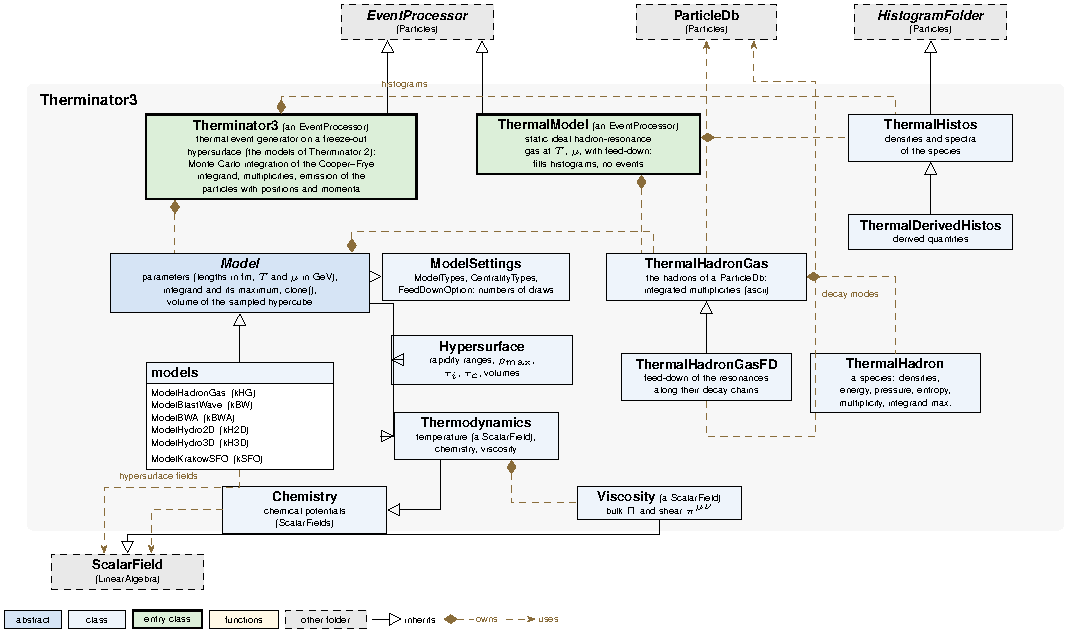
\includegraphics[width=\textwidth]{Therminator3Classes}
  \caption{Classes of Therminator3 (\code{models/Therminator3}): the generator task, the freeze-out models, the thermodynamic fields, the hadron gas, and the thermal model. Boxes: abstract classes (blue), classes (light blue), the entry classes of the folder (green), free functions (yellow), classes of other folders (grey, dashed). Open triangles point to the base class; dashed lines are dependencies, the diamond marking the owner.}
  \label{fig:therminator}
\end{figure*}

\paragraph{Emission.}
Hadrons are emitted according to the Cooper--Frye formula,
\begin{align}
  E\frac{dN}{d^3p} & = \frac{g}{(2\pi)^3}\int_\Sigma d\Sigma_\mu(x)\,p^\mu f(x,p), \\
  f(x,p) & = \frac{1}{\exp\!\bigl[(p\cdot u(x) - \mu(x))/T(x)\bigr] \pm 1},
\end{align}
with Fermi--Dirac or Bose--Einstein statistics, where $u$ is the velocity of the fluid on the hypersurface $\Sigma$, $T$
its temperature, and $\mu = B\mu_B + I_3\mu_I + S\mu_S + C\mu_C$ the chemical potential of the hadron, of baryon number
$B$, isospin $I_3$, strangeness $S$ and charm $C$. The hadrons emitted are those of the particle database, except the
quarks, leptons and gauge bosons and the hadrons heavier than 2.5~GeV; photons are not emitted.

\paragraph{Generation.}
As in THERMINATOR~2, the generation has two steps. First, the mean multiplicity $\avg{N}$ of each hadron is the
integral of the Cooper--Frye formula over the hypersurface and the momenta, computed by Monte Carlo
(\code{NSamples} points, $10^5$ by default), which also gives the maximum of the integrand. Then, for each event, the
number of each hadron is drawn from a Poisson distribution of mean $\avg{N}$ (or a Gaussian, \code{FluctuationType}),
and each hadron is generated by accepting or rejecting points of the integrand, drawn at random, against its maximum
times a safety factor (\code{MaxIntegrandSafety}, 1.2): the accepted point gives both the momentum of the hadron and
its position of emission, in fm. The multiplicities can be written to a file and read back, so that the integration
is done once for a set of parameters. The hadrons are emitted as they are produced, resonances included; a
\code{ParticleDecayerTask} placed after Therminator3 decays them.

\paragraph{Freeze-out models.}
The model is chosen by the key \code{HYDRO\_MODEL:TYPE}. All models share the sampling of the integrand. A point of
the hypersurface is drawn uniformly in the coordinates that parametrise it, and the momentum is drawn as
$\pT = \zeta/(1-\zeta)$ with $\zeta$ uniform in $[0,1)$, the rapidity $y$ uniform over a range $Y$
(\code{pRapidityRange}), and the azimuth $\varphi_p$ uniform. The integrand is then
\begin{equation}
  I = \frac{g}{(2\pi)^3}\,\frac{\pT}{(1-\zeta)^2}\,(d\Sigma\cdot p)\,f(x,p),
  \label{eq:t3-integrand}
\end{equation}
where $1/(1-\zeta)^2 = d\pT/d\zeta$, $p = (m_T\cosh y,\ \pT\cos\varphi_p,\ \pT\sin\varphi_p,\ m_T\sinh y)$ and $m_T = \sqrt{m^2+\pT^2}$. The mean
multiplicity is $\avg{N} = V\avg{I}$, where $V$ is the volume of the sampled region of coordinates and momenta. The
models differ by the hypersurface, the measure $d\Sigma\cdot p$ and the fluid velocity $u$ that enters $p\cdot u$.
Positions are written as $x = (\tau\cosh\eta,\ \rho\cos\varphi,\ \rho\sin\varphi,\ \tau\sinh\eta)$, with the
spatial rapidity $\eta$ uniform over \code{sRapidityRange}.
\begin{itemize}
  \item \code{BW}, the blast wave. Emission occurs at a constant proper time $\tau$ (\code{TauI}) from a cylinder of radius
  $\rho_{\max}$, with a radial transverse velocity $v_T$ (\code{tVelocity}) that is the same everywhere:
  \begin{align}
    p\cdot u & = \gamma_T\bigl(m_T\cosh(\eta-y) \nonumber\\ & \quad - v_T\pT\cos(\varphi-\varphi_p)\bigr), \\
    d\Sigma\cdot p & = \tau\rho\, m_T\cosh(\eta-y),
  \end{align}
  with $\gamma_T = (1-v_T^2)^{-1/2}$.
  \item \code{HG}, a static fireball: the blast wave without flow, $v_T = 0$.
  \item \code{BWA}, the variants of the blast wave of THERMINATOR~2 (\code{Subtype} 2 to 6). The hypersurface is tilted
  in the $(\tau,\rho)$ plane, $\tau(\rho) = \tau_i + A\rho$ (\code{Amplitude}), so that
  \begin{equation}
    d\Sigma\cdot p = \tau\rho\bigl(m_T\cosh(\eta-y) - A\,\pT\cos(\varphi-\varphi_p)\bigr).
  \end{equation}
  The transverse velocity is either constant (subtypes 2 and 3) or rises with the radius as
  $v_T(\rho) = (\rho/\rho_{\max})/(v + \rho/\rho_{\max})$, with $v$ = \code{tVelocity} (subtypes 4 to 6; Eq.~(42) of
  Ref.~\cite{Chojnacki:2011hb}). In subtypes 3, 5 and 6 the emission is delayed by a time $\Delta$ drawn from an
  exponential distribution of mean \code{Delay}. In subtype 6, which is new in \CAP{}, the particle also streams
  freely during the delay, $\vec{x} \to \vec{x} + \Delta\,\vec{p}/E$.
  \item \code{SFO}, the Krak\'ow single freeze-out model~\cite{Broniowski:2001we}. Emission occurs on the hyperboloid
  $\tau^2 - \rho^2 = \tau_f^2$ (\code{TauC}), with the Hubble-like flow $u = x/\tau_f$ of the single freeze-out:
  \begin{align}
    p\cdot u & = \frac{m_T\,\tau\cosh(\eta-y) - \pT\rho\cos(\varphi-\varphi_p)}{\tau_f}, \\
    d\Sigma\cdot p & = \tau_f\,\rho\,(p\cdot u),
  \end{align}
  where $\tau = \sqrt{\tau_f^2+\rho^2}$ is the proper time of the emission point.
  \item \code{HYDRO2D}, a hypersurface of boost-invariant (2+1)-dimensional hydrodynamics. The surface is the distance
  $D(\zeta,\varphi)$ from the point $(\tau_i, 0)$ of the $(\tau,\rho)$ plane, so that $\tau = \tau_i + D\sin\zeta$ and
  $\rho = D\cos\zeta$. The fluid has a transverse velocity $v_T(\zeta,\varphi)$ at an azimuth $\varphi + \varphi_F$, and
  \begin{align}
    p\cdot u & = \gamma_T\bigl(m_T\cosh(y-\eta) \nonumber\\ & \quad - v_T\pT\cos(\varphi-\varphi_p+\varphi_F)\bigr), \\
    d\Sigma\cdot p & = D\,\tau\,\bigl[D\cos\zeta\,(m_T\sin\zeta\,C + \pT\cos\zeta\,c) \nonumber\\
    & \quad + \partial_\zeta D\,\cos\zeta\,(\pT\sin\zeta\,c - m_T\cos\zeta\,C) \nonumber\\
    & \quad + \partial_\varphi D\,\pT\,s\bigr],
  \end{align}
  with $C = \cosh(y-\eta)$, $c = \cos(\varphi-\varphi_p)$ and $s = \sin(\varphi-\varphi_p)$.
  \item \code{HYDRO3D}, a hypersurface of (3+1)-dimensional hydrodynamics. The parametrisation adds a polar angle
  $\theta$: $\tau = \tau_i + D\sin\theta\sin\zeta$, $\rho = D\sin\theta\cos\zeta$, and $\eta = D\cos\theta/\Lambda$. The
  fluid has transverse components $u_x$, $u_y$ and a longitudinal rapidity $Y_F$, so that
  \begin{align}
    p\cdot u & = \sqrt{1+u_x^2+u_y^2}\; m_T\cosh(Y_F-y) \nonumber\\
    & \quad - \pT\,(u_x\cos\varphi_p + u_y\sin\varphi_p),
  \end{align}
  and $d\Sigma\cdot p$ follows from the derivatives of $D$ with respect to the three angles (Ref.~\cite{Chojnacki:2011hb}).
\end{itemize}
In the hydrodynamic models a negative $d\Sigma\cdot p$, a particle entering the hypersurface, is set to zero, as is
common practice; with \code{BackFlow}, only those particles are kept. The parameters of the analytic models
(temperature, chemical potentials, radius, proper times, velocity, ranges of rapidity) are keys of the task, with
lengths in fm and temperatures and chemical potentials in GeV; their defaults are those of the blast wave of
THERMINATOR~2. The hydrodynamic hypersurfaces are read from the XML files of THERMINATOR~2: the distance $D$ and the
fluid velocity as functions of the angles, together with the temperature, chemical potentials and initial proper time
of the calculation, which override those of the configuration. The derivatives of the distance are read when the file
provides them, and computed otherwise.
\todo{the shear and bulk viscous corrections ($\delta f$, class \code{Viscosity}) and the negative-binomial
fluctuations of the multiplicities are not finished; describe them when they are.}

\paragraph{Validation and the thermal model.}
The tests of Therminator3 compare its mean multiplicities of pions, kaons, protons and $\Lambda$ for the blast wave
with those of THERMINATOR~2 (agreement within 2.5\%), and the multiplicities and mean $\pT$ of generated events
with their expected values; they check that hydrodynamic hypersurfaces built to equal the blast wave reproduce its
multiplicities, in 2+1 and 3+1 dimensions, and, when THERMINATOR~2 is installed, run a hypersurface of its library.
A second task, \code{ThermalModel}, computes the densities, energy densities, pressures and entropy densities of a
static ideal hadron-resonance gas at a given temperature and chemical potentials, with the feed-down of the
resonances to the stable hadrons through their decays, and fills histograms of them; it generates no events.
The densities are the series
$n = \frac{g\,m^2T}{2\pi^2}\sum_{k\ge1}(\mp1)^{k+1}\lambda^k K_2(km/T)/k$, with the fugacity $\lambda = e^{\mu/T}$ and the
upper sign for fermions, truncated at five terms. The feed-down to a stable hadron follows the decay chains of the
particle database, with the branching ratios normalized to one, as the decayer draws them.
\todo{$\mu_Q$ is not used by \code{ThermalHadron::calculateAllProperties}: add it or remove the key.}

% ---------------------------------------------------------------------------------------------------------------
\subsection{Pythia8}
\label{sec:pythia}

\code{PythiaEventGenerator} generates events with Pythia~8~\cite{Bierlich:2022pfr}, linked to \CAP{} when it is built
with Pythia (Section~\ref{sec:build}). The beams are set by their PDG codes and either the energy in the centre of mass
or the energies of the two beams (proton--proton at 2.7~TeV by default), and the seed by \code{SeedValue}. Three
presets set the many Pythia parameters of models of collective effects in small systems: QCD-based colour
reconnection (\code{UseQCDCR}, on by default), rope hadronisation (\code{UseRopes}) and string shoving
(\code{UseShoving}). Any other Pythia setting is passed verbatim, as a string, by the keys \code{Option0} to
\code{Option29}, applied after the presets so that they can modify them. The particles of each Pythia event are
copied into the event of the task with their momenta and production vertices: by default the final-state particles
only, without photons, neutrinos, quarks, gluons and gauge bosons, each of which can be kept on request. Decays are
those of Pythia, set by its own options. The particles whose PDG code is not in the particle database of \CAP{} are
skipped and counted.

% ---------------------------------------------------------------------------------------------------------------
\subsection{Herwig 7}
\label{sec:herwig}

\code{HerwigEventGenerator} runs Herwig~7~\cite{Bellm:2015jjp} in the job, linked to \CAP{} when it is built with
Herwig (Section~\ref{sec:external}). Herwig is configured as on its command line: \code{Herwig read} turns an input
file (\code{.in}) of repository commands into a run file (\code{.run}) holding the event generator, and \code{Herwig
run} generates its events. The task does both. Given an input file (\code{InputFile}, or a \code{.in} file given as
\code{RunFile}), it reads it, in the directory of the file and with the repository \code{Repository}
(\code{HerwigDefaults.rpo} by default), unless the run file that the input saves is already there and is newer;
otherwise it loads the run file \code{RunFile}. Commands applied to the generator before the run, as by \code{Herwig
run -x}, come from a file (\code{SetupFile}) and from the keys \code{Option0} to \code{Option19}, for instance
{\small
\begin{verbatim}
set /Herwig/Generators/EventGenerator:
    EventHandler:LuminosityFunction:Energy 13600.0
set /Herwig/Particles/pi0:Stable Stable
\end{verbatim}
}
so that the beam energy, or the decays, can be changed without a new run file. The seed is set by \code{SeedValue}
(with \code{SetSeed}), and \code{Tag} is appended to the names of the log and output files that Herwig writes.
Processes integrated by Matchbox need their grids first, made by \code{Herwig build} and \code{Herwig integrate} on
the command line. Each Herwig event is generated by \code{execute()}, and its final-state particles are copied into
the event of the task with their momenta (GeV) and production vertices (mm): photons and neutrinos are included unless
\code{SavePhotons} or \code{SaveNeutrinos} is off, and a particle is added when it passes the first particle filter of
the task. As for Pythia, the particles whose PDG code is not in the particle database are skipped and counted.
Herwig's events are unweighted by default; weighted events, whose weight \CAP{} events cannot carry, are counted and
reported, together with the events that Herwig failed to generate. At the end of the job, the task reports the cross
section and Herwig writes its output file. Since Herwig keeps a global state, a job has a single
\code{HerwigEventGenerator}. On macOS, Herwig and ThePEG must be built with \code{-fno-typed-cxx-new-delete} and linked
to \code{libc++}, as is the \CAP{} module.

% ---------------------------------------------------------------------------------------------------------------
\subsection{Event readers}
\label{sec:readers}

Readers take the events produced by other generators from their files, found from the key \code{DataImportPath}
(the environment variable \code{CAP\_DATA\_IMPORT\_PATH} by default) and the name or pattern \code{DataImportFile}.
Particles whose PDG code is not in the particle database are skipped, and counted in the report of the task at the
end of the job.
\begin{itemize}
  \item \code{PythiaEventReader} reads Pythia events stored in ROOT trees of \code{TParticle} objects (key
  \code{TreeName}), a set of files being read as one chain; the particles kept are selected as by the generator.
  \item \code{EposEventReader} reads the ROOT trees written by EPOS~\cite{Werner:2010aa} (key \code{TreeName}), a set
  of files being read as one chain: per event, the number of particles, the impact parameter, and the PDG codes and
  momenta of the particles, whose energies are computed from the masses of the database.
  \item \code{PHSDEventReader} reads the text files of PHSD~\cite{Cassing:2009vt}: a file, or the files matching
  \code{DataImportFile} (\code{*.dat} by default) in a directory and its sub-directories, read in order. Each event
  has a header with the impact parameter, the colliding nuclei, the energy, the number of participants and the
  event-plane angles and eccentricities of orders 2 to 5, followed by the PDG codes, charges, momenta and energies of
  the particles; the particles keep the energies of the file, since PHSD particles may be off their mass shell.
\end{itemize}
\todo{the program writing the Pythia ROOT trees read by \code{PythiaEventReader} is not part of \CAP{}: say where
it comes from.}

% ---------------------------------------------------------------------------------------------------------------
\subsection{Glauber model}
\label{sec:glauber}

\paragraph{Class structure.}
The Monte Carlo Glauber model~\cite{Miller:2007ri} of \CAP{} derives from TGlauberMC, the PHOBOS Glauber Monte
Carlo~\cite{Alver:2008aq}. The task \code{GlauberGenerator} makes the events: for each event, it places the
nucleons of the two nuclei (\code{GlauberNucleus}, of a type \code{GlauberNucleusType} taken from the database
\code{GlauberDb}, with the radial densities of \code{NuclearDistribution}), draws the impact parameter, and finds
the binary and hard nucleon--nucleon collisions, with the collision profiles (\code{NNProfile},
\code{NucleonProfile}, \code{SmearingProfile}, \code{PTotProfile}) and the inelastic cross section
(\code{NNXSectVsSqrtS}). An event (\code{GlauberEvent}) holds the two nuclei, the impact parameter and the numbers
of participants, binary collisions and spectators. The task \code{GlauberAnalyzer} computes the moments of the
participants (\code{GlauberEventMoments}) and fills the histograms of \code{GlauberHistos} for each event filter
(\code{GlauberEventFilter}). Figure~\ref{fig:glauber} shows the classes of the folder.

\begin{figure*}[t]
  \centering
  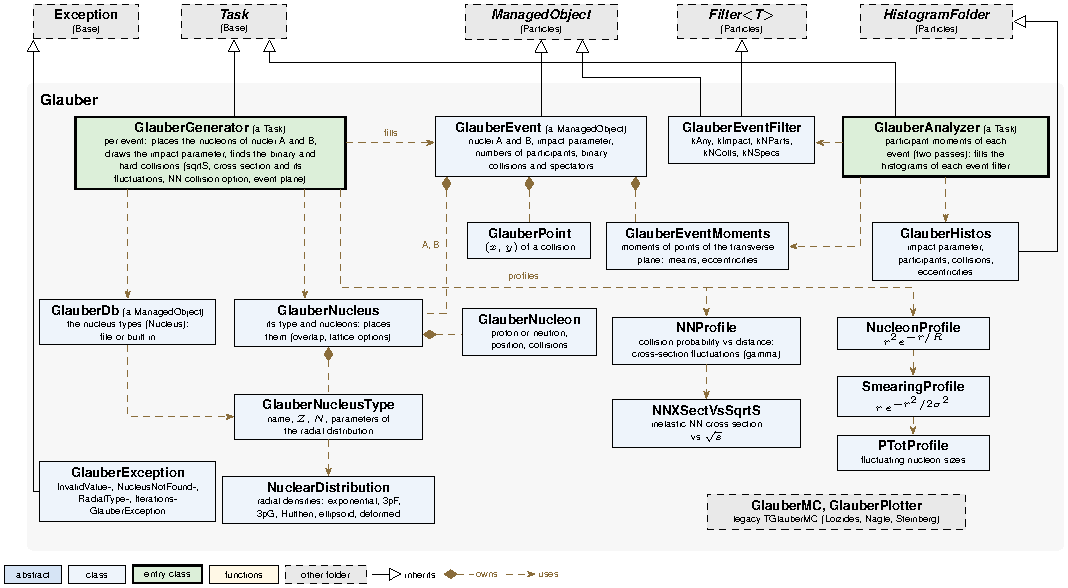
\includegraphics[width=\textwidth]{GlauberClasses}
  \caption{Classes of the Glauber model (\code{models/Glauber}). Boxes: abstract classes (blue), classes (light blue), the entry classes of the folder (green), free functions (yellow), classes of other folders (grey, dashed). Open triangles point to the base class; dashed lines are dependencies, the diamond marking the owner.}
  \label{fig:glauber}
\end{figure*}

\todo{to come later: event generation and analysis.}

% Section: CapGui
\section{CapGui}
\label{sec:capgui}

\subsection{Windows, canvases and graphs}
\label{sec:windows}

\todo{several windows, several canvases per window, several graphs per canvas; the data browser next to the display.}

\subsection{Fits}
\label{sec:guifits}

\todo{fits in one and two variables; simple and composite parameterised functions; ranges and regions; the residual panel and the Fits pane.}

% Section: Example applications
\section{Example applications}
\label{sec:examples}

\subsection{Proton--proton collisions with Pythia8}
\label{sec:example-pythia}

\todo{pp at 13.7 TeV: $R_2$, $P_2$ and balance functions; the XML workflow and the figures.}

\subsection{A thermal model with Therminator3}
\label{sec:example-therminator}

\todo{a scan of filters.}

\subsection{A performance study}
\label{sec:example-performance}

\todo{smearers and efficiencies.}

% Section: Performance and validation
\section{Performance and validation}
\label{sec:validation}

\subsection{Timing}
\label{sec:timing}

\todo{events per second for typical analyses.}

\subsection{Validation}
\label{sec:checks}

\todo{comparisons with known results and analytic cases; the test suite run by ctest.}

% Section: Summary and outlook
\section{Summary and outlook}
\label{sec:summary}

\todo{what CAP 8 provides; planned work (Glauber analyses, flattenicity, anisotropic flow, removing the last uses of ROOT).}


\appendix
% Appendix: Configuration keys of an analysis task
\section{Configuration keys of an analysis task}
\label{app:xml}

\todo{the keys of a typical analysis task (filters, HISTOGRAM group, SOURCE\_TASK), with an excerpt of a workflow.}

% Appendix: The binary format
\section{The binary format}
\label{app:binary}

\todo{the layout of a CAP file record by record; the encoding of each streamable class; version rules.}

% Appendix: Installation on macOS and Linux
\section{Installation on macOS and Linux}
\label{app:install}

\todo{step-by-step recipes for macOS and Linux.}


\bibliographystyle{unsrtnat}
\bibliography{refs}

\end{document}
